\documentclass[11pt,letterpaper]{article}

% Compile from the folder containing this file.
% This path works in template/ and in sibling course folders.
% Shared formatting for course notes. Loaded by each course's main.tex.
\usepackage[T1]{fontenc}
\usepackage[utf8]{inputenc}
\usepackage{lmodern}
\linespread{1.15}
\usepackage[margin=1in]{geometry}
\usepackage{amsmath,amssymb,amsthm}
\usepackage{mathtools}
\usepackage{graphicx}
\usepackage{booktabs}
\usepackage{enumitem}
\usepackage{xcolor}
\usepackage{hyperref}
\usepackage{tikz}
\usetikzlibrary{decorations.pathreplacing,positioning}
\usepackage{xparse}
\usepackage{etoolbox}

\hypersetup{colorlinks=true,linkcolor=blue!50!black,urlcolor=blue!50!black}
\setlength{\parindent}{0pt}
\setlength{\parskip}{0.5em}
\setlist{nosep}

% Unnumbered section headings: entries show as "Week 1", not "1 Week 1",
% both in the body and in the table of contents.
\setcounter{secnumdepth}{0}

% Each \section (i.e. each week's entry) starts on its own new page. The
% \newpage that used to follow \tableofcontents in each course's main.tex
% is redundant now and has been removed, so week 1 isn't pushed to a blank
% page by this.
\pretocmd{\section}{\newpage}{}{\errmessage{Failed to patch \string\section}}

% Tracks whether \section was the most recent sectioning/lecture command,
% so a \newlecture immediately following a \section (the usual "week's
% first lecture" case) doesn't also throw in its own \newpage, which would
% otherwise leave a blank page between the two. Set true by \section, and
% cleared by \newlecture whether or not it was true, so it only fires for
% a \newlecture that directly follows a \section (nothing else in between).
\newbool{newlecture@justsection}
\pretocmd{\section}{\booltrue{newlecture@justsection}}{}{\errmessage{Failed to patch \string\section}}

% Custom head format: bold, unparenthesized title, with a \quad gap after
% the number (e.g. "Theorem 3.2  Distribution" instead of "Theorem 3.2
% (Distribution)."), reusing amsthm's usual spacing/punctuation otherwise.
% When a title is given, the body text starts on its own new line below the
% head instead of running inline after it; untitled (auto-numbered-only)
% instances stay inline as usual. Body text is upright (not italic) for all
% six environments. Two variants share this head format but differ in
% end-of-head punctuation: theorem/lemma/proposition/exercise keep a
% trailing period, definition/example drop it (no period after the title).
\makeatletter
\newcommand{\thmpunct}{.}
\newtheoremstyle{boldhead}{}{}{\normalfont}{}{\bfseries}{\thmpunct}{5pt plus 1pt minus 1pt}%
    {\thmname{#1}\thmnumber{\@ifnotempty{#1}{ }#2}\thmnote{\@ifnotempty{#3}{\quad#3}}%
     \@ifnotempty{#3}{\def\thmheadnl{\newline}\thm@headsep\z@skip}{}}
\newtheoremstyle{boldheadnp}{}{}{\normalfont}{}{\bfseries}{}{5pt plus 1pt minus 1pt}%
    {\thmname{#1}\thmnumber{\@ifnotempty{#1}{ }#2}\thmnote{\@ifnotempty{#3}{\quad#3}}%
     \@ifnotempty{#3}{\def\thmheadnl{\newline}\thm@headsep\z@skip}{}}
\makeatother

\theoremstyle{boldhead}
\newtheorem{theorem}{Theorem}
\newtheorem{lemma}[theorem]{Lemma}
\newtheorem{proposition}[theorem]{Proposition}
\newtheorem{corollary}[theorem]{Corollary}
\newtheorem{exercise}[theorem]{Exercise}
\theoremstyle{boldheadnp}
\newtheorem{definition}[theorem]{Def.}
\newtheorem{example}[theorem]{Example}
\theoremstyle{remark}
\newtheorem*{remark}{Remark}

% \begin{theorem}[Title][2.7]: both optional arguments are new on top of
% the environments' usual single bracket. The first argument still behaves
% exactly like plain amsthm's optional title (existing notes using
% \begin{example}[Some Name] etc. are unaffected). The second argument, if
% given, overrides the displayed number (e.g. to match a textbook's own
% numbering) instead of the shared theorem counter's automatic value; the
% counter itself still advances normally, so later auto-numbered
% environments are unaffected too.
\newcommand{\addtitleandnumber}[1]{%
    \csletcs{#1orig}{#1}%
    \csletcs{end#1orig}{end#1}%
    \RenewDocumentEnvironment{#1}{o o}{%
        \IfValueT{##2}{\ifblank{##2}{}{\renewcommand{\thetheorem}{##2}}}%
        \IfValueTF{##1}{\ifblank{##1}{\csname#1orig\endcsname}{\csname#1orig\endcsname[##1]}}{\csname#1orig\endcsname}%
    }{\csname end#1orig\endcsname}%
}
\addtitleandnumber{theorem}
\addtitleandnumber{lemma}
\addtitleandnumber{proposition}
\addtitleandnumber{corollary}
\addtitleandnumber{definition}
\addtitleandnumber{example}
\addtitleandnumber{exercise}

% Common mathematical notation.
\newcommand{\R}{\mathbb{R}}
\newcommand{\N}{\mathbb{N}}
\newcommand{\Z}{\mathbb{Z}}
\newcommand{\E}{\mathbb{E}}
\newcommand{\Prob}{\mathbb{P}}
\DeclareMathOperator{\Var}{Var}
\DeclareMathOperator{\Cov}{Cov}

% \newlecture[title][date]: bold, centered marker for the start of a new
% lecture. Both arguments are optional. Numbering runs continuously across
% the whole document (i.e. across all weeks' entries, not reset per
% \section), so the Nth \newlecture in the course is always "Lecture N".
% Each lecture starts on its own new page, except when it directly follows
% a \section heading (which already started a new page of its own), so the
% two stay together instead of leaving a blank page in between.
\newcounter{lecture}
\renewcommand{\thelecture}{\arabic{lecture}}
% Set \lecturetoctrue in a course's main.tex to list each lecture as a
% top-level table-of-contents entry ("Lecture N: title", or the date when
% untitled), with \subsection headings nested beneath it.
\newif\iflecturetoc
\NewDocumentCommand{\newlecture}{o o}{%
    \stepcounter{lecture}%
    \ifbool{newlecture@justsection}{}{\newpage}%
    \boolfalse{newlecture@justsection}%
    \iflecturetoc
        \phantomsection
        \addcontentsline{toc}{section}{Lecture \thelecture\IfValueTF{#1}{\ifblank{#1}{\IfValueT{#2}{\ifblank{#2}{}{ (#2)}}}{: #1}}{\IfValueT{#2}{\ifblank{#2}{}{ (#2)}}}}%
    \fi
    \par\vspace{1em}
    \begin{center}
        \textbf{\Large Lecture \thelecture\IfValueT{#1}{: #1}}\\[2pt]
        \IfValueT{#2}{\normalsize #2}
    \end{center}
    \vspace{0.5em}%
}

% Handwritten-note-style helpers: red definition labels, blue margin
% annotations, yellow highlights, underlined mini-headers.
\newcommand{\deflabel}[2]{\par\noindent{\color{red!70!black}\textbf{Def #1}}\quad\textbf{#2}\par\nobreak}
\newcommand{\exlabel}[2]{\par\noindent\textbf{Example #1}\quad\textbf{#2}\par\nobreak}
\newcommand{\heading}[1]{\par\noindent{\color{red!70!black}\textbf{#1}}\par}
\newcommand{\header}[1]{\par\vspace{0.5em}\noindent\textbf{#1}\par\vspace{-0.2em}}
\newcommand{\aside}[1]{\ifmmode{\color{blue!55!black}\text{\itshape #1}}\else{\color{blue!55!black}\itshape #1}\fi}
\newcommand{\hly}[1]{\colorbox{yellow!55}{$#1$}}
\newcommand{\hlt}[1]{\colorbox{yellow!55}{#1}}
% \boldmath makes any math the argument switches into (e.g. \rb{$r$}) use
% the bold math version automatically, so callers don't need to manually
% wrap math content in \boldsymbol{}.
\newcommand{\rb}[1]{{\color{red!70!black}\boldmath\textbf{#1}}}
\renewcommand{\b}[1]{\textbf{#1}}
\definecolor{navy}{RGB}{0,32,96}
\newcommand{\dbb}[1]{{\color{navy}\textbf{#1}}}
\newcommand{\db}[1]{{\color{navy}#1}}

% Wider padding inside \boxed{} equations (default \fboxsep is 3pt).
% Scoped to \boxed only, so \colorbox highlights (e.g. \hly) are unaffected.
\let\oldboxed\boxed
\renewcommand{\boxed}[1]{{\setlength{\fboxsep}{10pt}\oldboxed{#1}}}


% Replace these details for each course.
\newcommand{\coursecode}{CHE374}
\newcommand{\coursename}{Economic Analysis and Decision Making}
\newcommand{\term}{Fall 2026}
\newcommand{\studentname}{Bonnie Zhuang}

\title{\coursecode{} --- \coursename\\[0.5em]\large Course Notes}
\author{\studentname}
\date{\term}

% CHE374-only override: definitions are unnumbered, shown as
% "Definition - <term>" in bold red instead of the shared numbered style,
% with the definition body indented so it's clearly set off from the header.
\makeatletter
\renewenvironment{definition}[1][]{%
    \par\noindent
    \def\@defterm{#1}%
    \ifx\@defterm\@empty
        \noindent\textbf{Definition}%
    \else
        \noindent\textbf{Definition - \textcolor{red}{\@defterm}}%
    \fi
    \par\nobreak
    \begin{list}{}{\leftmargin=1.5em \itemindent=0pt \listparindent=0pt \parsep=\parskip \topsep=0pt \itemsep=0pt}
    \item\relax
}{%
    \end{list}
    \vspace{0.5em}
}
\makeatother

% CHE374-only override: \heading is black and bold instead of the shared
% template's red.
\renewcommand{\heading}[1]{\par\noindent\textbf{#1}\par}

% CHE374-only override: examples are unnumbered, shown as just "Example"
% (or "Example  <Title>" when a title is given) instead of the shared
% numbered style, and the body always starts on a new line below the head.
\makeatletter
\RenewDocumentEnvironment{example}{o}{%
    \par\noindent\textbf{Example\IfValueT{#1}{\ifblank{#1}{}{\quad#1}}}%
    \par\nobreak
}{%
    \par\vspace{0.5em}%
}
\makeatother

% CHE374-only: \topic{title} replaces \newlecture. Topics are numbered
% within each week ("1.1 - Interest Rate"), resetting at every \section.
% secnumdepth=0 stops \section from stepping its own counter, so the week
% number is tracked separately by patching \section.
\newcounter{week}
\newcounter{topic}[week]
\pretocmd{\section}{\stepcounter{week}}{}{\errmessage{Failed to patch \string\section}}
\newcommand{\topic}[1]{%
    \stepcounter{topic}%
    \phantomsection
    \subsection*{\theweek.\arabic{topic} - #1}%
    \addcontentsline{toc}{subsection}{\theweek.\arabic{topic} - #1}%
}

\begin{document}
\maketitle
\tableofcontents
\setcounter{week}{0} % \tableofcontents's \section* also stepped it

% Add one input per lecture, in the order you want them to appear.
% !TeX root = ../main.tex

% Edit this title for each week's entry.
\section{Week 1 - Introduction and Time Value of Money}

\topic{Interest Rate}

\heading{Engineering Project Life Cycles}
\begin{itemize}
    \item All engineering projects have a life cycle:
    \begin{itemize}
        \item Conceptualization $\to$ detailed economic analysis $\to$ go / no go decision $\to$ design $\to$ build $\to$ utilize / produce $\to$ phase out / dispose
    \end{itemize}
    \item Most of the project's cost is \dbb{committed early}, during conceptual and detailed design, even though the money is mostly \dbb{spent later} (production, operation)
    \item We \rb{invest} in projects to gain benefits (economic and societal)
\end{itemize}

\begin{center}
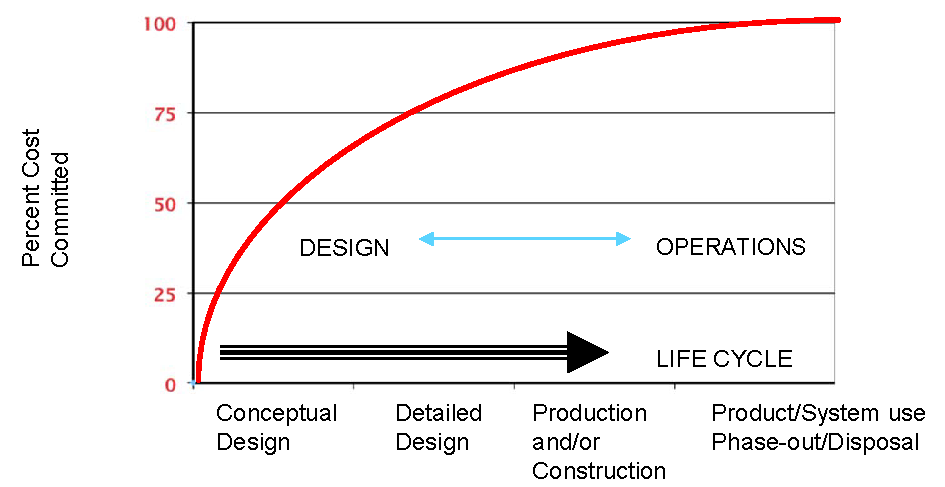
\includegraphics[width=0.75\linewidth]{figures/life_cycle_cost.png}
\\[2pt] \textit{\small Most cost is committed early, during design, before it is actually spent}
\end{center}

\heading{Time Value of Money}
\begin{itemize}
    \item Borrowing (renting) money has a cost for the \b{borrower}, thus lending money \textit{should} create value for the lender (investor/creditor)
    \item Costs and benefits occur in different time periods
    \item The cost/benefit today to the future is compared by \rb{interest}
\end{itemize}

\begin{example}
    You borrow \$10 from a lender today and return it a year later.
    \begin{itemize}
        \item You must return the \$10 borrowed $\Rightarrow$ the \rb{principal}
        \item The lender charges an extra amount, e.g.\ \$1 $\Rightarrow$ the \rb{interest}
        \item The \rb{interest rate} is interest/principal:
        \[i = \frac{1}{10} = 10\%\]
    \end{itemize}
\end{example}

\heading{Present and Future Worth}
\[P = \text{ present worth/\rb{Principal}} \qquad F=\text{ future worth} \qquad i=\text{ interest rate}\]
\[F = P+Pi \qquad F = P(1+i)\]

\begin{center}
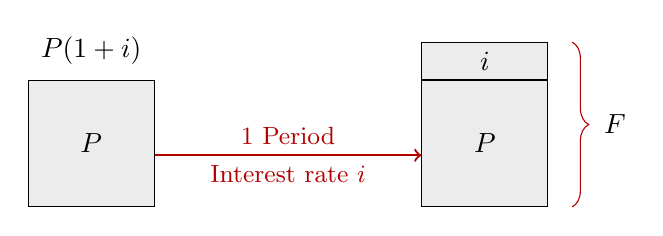
\begin{tikzpicture}[
    box/.style={draw, fill=gray!15, minimum width=1.6cm, minimum height=1.6cm},
    ibox/.style={draw, fill=gray!15, minimum width=1.6cm, minimum height=0.4cm},
    lbl/.style={red!70!black, font=\small}
]
    % Present worth box
    \node[box] (P) at (0,0) {$P$};
    \node[above=2pt of P] {$P(1+i)$};

    % Future worth: P portion and interest portion stacked
    \node[box, minimum height=1.6cm] (F) at (5,0) {$P$};
    \node[ibox, above=0pt of F] (I) {$i$};

    % Arrow between them
    \draw[->, thick, red!70!black] ([yshift=-0.15cm]P.east) -- ([yshift=-0.15cm]F.west)
        node[midway, above, lbl] {1 Period}
        node[midway, below, lbl] {Interest rate $i$};

    % Brace marking total future worth F
    \draw[decorate, decoration={brace, amplitude=6pt}, red!70!black]
        ([xshift=0.3cm]I.north east) -- ([xshift=0.3cm]F.south east)
        node[midway, right=8pt, black] {$F$};
\end{tikzpicture}
\end{center}
\begin{itemize}
    \item A \dbb{higher} payoff ($F$) is expected as $i$ increases
    \item For a given $F$ with increased $i$, $P$ \dbb{decreases}
\end{itemize}


\heading{Interest Rate}
\begin{itemize}
    \item Expressed as \%
    \item Vary widely over time and different types of investments.
    \begin{itemize}
        \item A \b{T-Bill} (Treasury Bill, short term loan to the Bank of Canada) will earn the \dbb{lowest} rate of return, as it's considered "risk-free"
        \item Canadian and provincial bonds pay typically \dbb{slightly higher} interest rates
        \item Personal/small business loans are much riskier and earn \dbb{significantly higher} interest rates
    \end{itemize}
\end{itemize}

\heading{Factors that Affect Interest Rates}
\begin{itemize}
    \item \b{Inflation}: prices generally tend to increase over time. Higher expected inflation generally leads to \dbb{higher interest rates}
    \item \b{Credit (default) Risk}: associated with the borrower being able to pay back interest and principal. Higher risk of default $\Rightarrow$ \dbb{higher interest rates}
    \item \b{Liquidity Risk}: associated with being able to access the invested funds during the investment. The less liquid the investment (greater the risk), the \dbb{higher the interest rate}
    \item \b{Maturity Risk}: associated with the time horizon. Longer the maturity, longer payoff, increases credit (and potential liquidity) risk $\Rightarrow$ \dbb{higher interest rates}
\end{itemize}
\db{Generally, as \dbb{risk} increases, the \dbb{interest rate} increases.}

\begin{example}
    What would the impact be expected on the interest rate associated with a large new mining project under the following scenarios, and how would the current value be impacted?
    \begin{itemize}
        \item The expected time to complete the project construction increases
        \\\db{Interest rate will increase as the maturity risk is directly incrased, raising risks of liquidity and credit. The present value would then decrease, from both the interest rate increasing and the time horizon increasing.}
        \item The estimate amount of ore available to be mined increases
        \\\db{The future cash flow would increase, thus the value of the project will increase, decreasing risk. Credit risk will drop but not others.}
    \end{itemize}
\end{example}

\heading{Summary}
\begin{itemize}
    \item \rb{Interest} is money earned by investors for allowing others to use their money
    \item The \rb{interest rate} is a rate at which interest is earned.
    \item The interest rate is determined by \dbb{risks} associated with the investment.
\end{itemize}





\topic{Simple and Compound Interest}

\heading{Present and Future Worth}
\[P = \text{ amount of money today (principal)} \qquad F_N = \text{ future amount in year }N\]
\[i = \text{ interest rate} \qquad I\text{ = interest amount}\]
\[F = P+I \qquad F_1 = P+Pi\]

\begin{example}[GIC]
    You deposit \$5,000 in the bank for 1 year as a \b{Guaranteed Investment Certificate (GIC)}, i.e.\ you \textit{lent} the bank the money for a fixed time period. After 1 year the bank pays 10\% interest.
    \\\db{You get $I = 5000(0.10) = \$500$ as ``rent'' for lending the \$5,000, and the \$5,000 is also returned.}
    \begin{itemize}
        \item This is a \rb{simple} interest loan: you receive the money when the GIC \b{matures}
        \item \b{Matures}: the borrower must pay the loan back
    \end{itemize}
\end{example}

\heading{Simple vs Compound Interest}
\begin{itemize}
    \item \rb{Simple} applies \dbb{only to the original principal} (GIC, aka Certificate of Deposit (CD) in the U.S.)
    \item \rb{Compound} interest applies to the \dbb{principal AND all interest already accrued} (mortages, credit card debt...)
    \item Assume \dbb{compound} unless stated otherwise
\end{itemize}

\heading{Simple Interest}
\begin{tabular}{c|c|c|c}
    Beginning of Period & Amount Lent & Interest Amount & Amount Owed at Period End \\\hline
    1 & $P$ & $Pi$ & $P+Pi$ \\
    2 & $P+Pi$ & $Pi$ & $P+2Pi$ \\
    3 & $P+2Pi$ & $Pi$ & $P+3Pi$ \\
    ... & ... & ... & ... \\
    $N$ & $P+(N-1)Pi$ & $Pi$ & $P+NPi = P(1+Ni)$
\end{tabular}
\[\boxed{\begin{gathered}
    F_N = P(1+Ni)\\[4pt]
    \begin{array}{@{}l@{}}
        F_N: \text{amount owed after } N \text{ periods}\\
        P: \text{principal}\\
        i: \text{interest rate per period}\\
        N: \text{number of periods}
    \end{array}
\end{gathered}}\]

\heading{Compound Interest}
\begin{tabular}{c|c|c|c}
    Beginning of Period & Amount Lent & Interest Amount & Amount Owed at Period End \\\hline
    1 & $P$ & $Pi$ & $P(1+i)$ \\
    2 & $P(1+i)$ & $P(1+i)i$ & $P(1+i)^2$ \\
    3 & $P(1+i)^2$ & $P(1+i)^2 i$ & $P(1+i)^3$ \\
    ... & ... & ... & ... \\
    $N$ & $P(1+i)^{N-1}$ & $P(1+i)^{N-1}i$ & $P(1+i)^N$
\end{tabular}
\[\boxed{\begin{gathered}
    F_N = P(1+i)^N\\[4pt]
    \begin{array}{@{}l@{}}
        F_N: \text{amount owed after } N \text{ periods}\\
        P: \text{principal}\\
        i: \text{interest rate per period}\\
        N: \text{number of periods}
    \end{array}
\end{gathered}}\]

\begin{example}[Simple Interest]
    If you borrow \$100 for 3 years at 10\% annual interest (simple interest), how much interest will you pay, and how much will you owe after 3 years?
    \[P = 100 \qquad i = 10\% \qquad N = 3\]
    \begin{align*}
        I &= NPi = 3(100)(0.10) = \db{\$30}\\
        F_3 &= P + NPi = 100 + 30 = \db{\$130}
    \end{align*}
\end{example}

\begin{example}[Compound Interest]
    If you borrow \$100 for 3 years at 10\% annual interest (compound interest), how much interest will you pay, and how much will you owe after 3 years?
    \begin{align*}
        F_3 &= P(1+i)^N = 100(1.10)^3 = \db{\$133.10}\\
        I &= F_3 - P = 133.10 - 100 = \db{\$33.10}
    \end{align*}
    \db{The extra \$3.10 compared to simple interest is interest earned on interest.}
\end{example}

\heading{Simple Interest is Linear, Compound Interest is Exponential}
\begin{center}
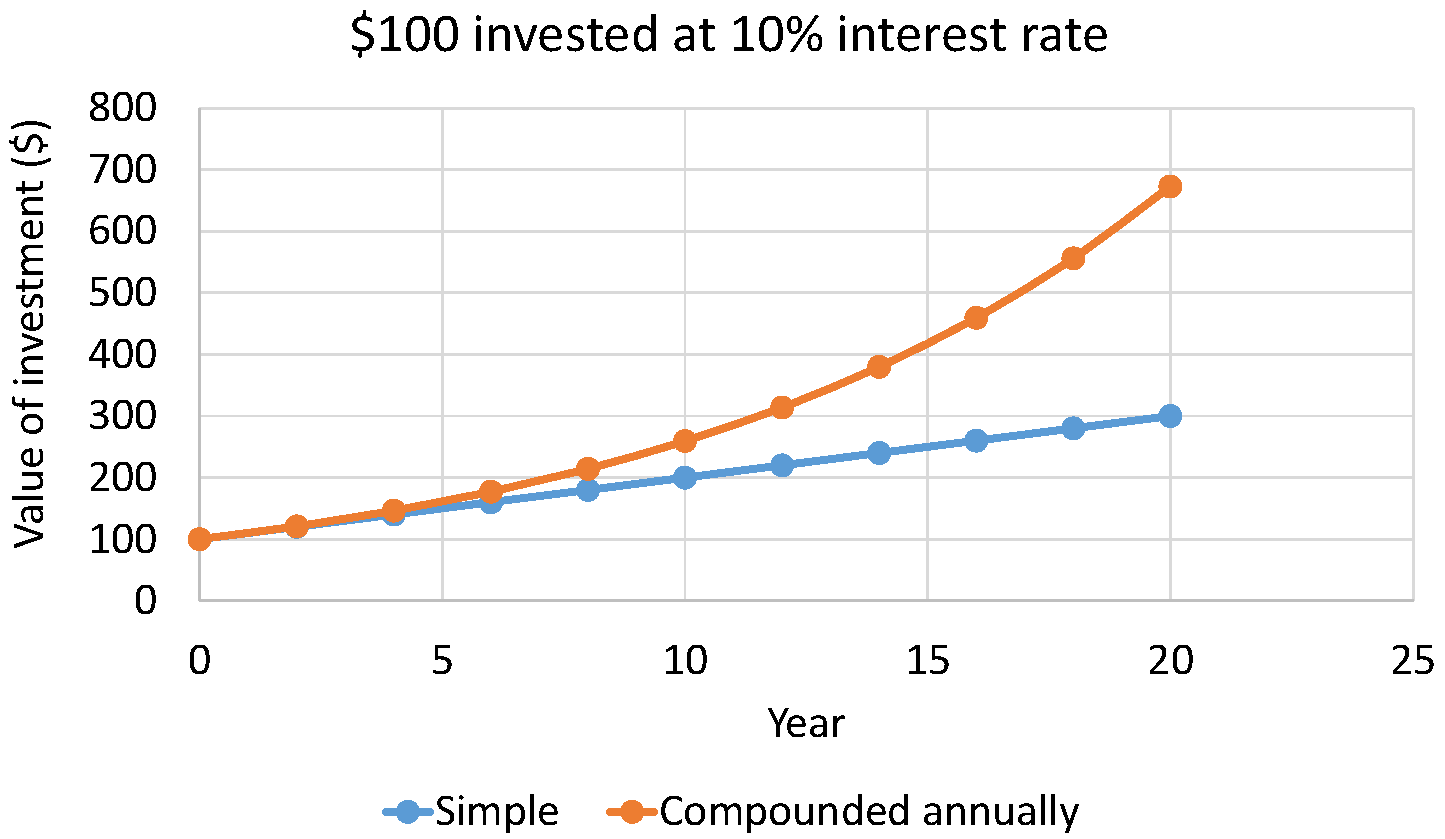
\includegraphics[width=0.7\linewidth]{figures/simple_vs_compound.png}
\\[2pt] \textit{\small \$100 invested at 10\%: \$300 (simple) vs.\ \$673 (compound) after 20 years}
\end{center}

\begin{example}[The Power of Compounding]
    The Dutch West India Company (supposedly) paid \$24 to purchase Manhattan Island in 1626. If the company had invested the \$24 in a savings account that earned 7\% interest per year, how much would it be worth today (2020, $N = 394$)?
    \begin{align*}
        \text{Simple: } F &= 24 + 394(24)(0.07) \approx \db{\$686}\\
        \text{Compound: } F &= 24(1.07)^{394} \approx \db{\$9{,}066{,}082{,}143{,}625}
    \end{align*}
    \begin{center}
    \begin{tabular}{c|r|r}
        Year & Simple (7\%) & Compound (7\%) \\\hline
        1626 & \$24 & \$24 \\
        1676 & \$108 & \$707 \\
        1726 & \$192 & \$20,825 \\
        1776 & \$276 & \$613,448 \\
        1826 & \$360 & \$18,070,359 \\
        1876 & \$444 & \$532,299,016 \\
        1926 & \$528 & \$15,679,945,443 \\
        1976 & \$612 & \$461,884,545,916 \\
        2020 & \$686 & \$9,066,082,143,625
    \end{tabular}
    \end{center}
\end{example}

\heading{Summary}
\begin{itemize}
    \item Simple Interest: $F_N = P+NPi$
    \item Compound Interest: $F_N = P(1+i)^N$
    \item Remember: \rb{interest rate} $=$ interest/principal
\end{itemize}




\topic{Subperiod Compounding \& Effective Interest Rates}

\heading{Compound Interest}
\begin{itemize}
    \item Recall: \rb{compound} interest applies to the principal AND to all interest already accrued
    \item ``To compound'' (verb) is to reinvest the principal PLUS the interest and earn interest on both:
    \[F = P(1+i)^N\]
\end{itemize}

\heading{Compound Multiple Times per Year}
\begin{itemize}
    \item \rb{$r$}: \b{nominal interest rate} (usually for 1 year)
    \item \rb{$m$}: times compounded in a year, aka \b{subperiods}
    \item \rb{$i_s$}: \b{subperiod interest rate}
\end{itemize}
\[\boxed{\begin{gathered}
    i_s = \frac{r}{m}\\[4pt]
    \begin{array}{@{}l@{}}
        i_s: \text{subperiod interest rate}\\
        r: \text{nominal interest rate (usually per year)}\\
        m: \text{number of subperiods per year}
    \end{array}
\end{gathered}}\]

\begin{example}
    You lend \$100. The nominal interest rate is 6\%.
    \\What is the total amount in the account at the end of the year if the compounding period is
    \[P = 100 \qquad r = 6\%\]
    \begin{enumerate}[label = \alph*)]
        \item 1 year:
        \begin{align*}
            F &= P(1+r)\\
            &=100(1+0.06)\\
            &=106
        \end{align*}
        \item 3 months:
        \[m = 4 \quad \Rightarrow \quad i_s = \frac{r}{m} = \frac{0.06}{4} = 0.015\]
        \begin{align*}
            F &= P(1+i_s)^m\\
            &=100(1+0.015)^4\\
            &=106.14
        \end{align*}
    \end{enumerate}
\end{example}

\begin{example}[Reflection]
    True or false: for the same nominal interest rate, the more frequently you compound, the more you earn at the end of the year.
    \\\db{True. Each extra compounding lets earlier interest start earning interest sooner (\$106 vs.\ \$106.14 above). The gain shrinks as $m$ grows, though, approaching a finite limit (continuous compounding).}
\end{example}

\heading{Effective Interest Rate}
\begin{itemize}
    \item How do we compare investments with different compounding periods?
    \item \rb{$i_e$}: \b{effective interest rate}, the equivalent interest rate of an account that is compounded just \dbb{once} over the stated time period (usually 1 year)
    \item Set one year of subperiod compounding equal to one compounding at $i_e$:
    \[P(1+i_e) = P\left(1+\frac{r}{m}\right)^m\]
\end{itemize}
\[\boxed{\begin{gathered}
    i_e = \left(1+\frac{r}{m}\right)^m - 1\\[4pt]
    \begin{array}{@{}l@{}}
        i_e: \text{effective interest rate (per year)}\\
        r: \text{nominal interest rate (per year)}\\
        m: \text{number of subperiods per year}
    \end{array}
\end{gathered}}\]

\begin{example}
    Which account earns you more money after 1 year?
    \begin{itemize}
        \item Option A: $r = 6\%$, compounded monthly
        \item Option B: $r = 6.3\%$, compounded once a year
    \end{itemize}
    \begin{align*}
        \text{A: } i_e &= \left(1+\frac{0.06}{12}\right)^{12} - 1 = (1.005)^{12} - 1 = 6.17\%\\
        \text{B: } i_e &= r = 6.3\% \quad (m = 1)
    \end{align*}
    \db{Option B earns more, since $6.3\% > 6.17\%$. Compare the \dbb{effective} rates, not the nominal ones.}
\end{example}

\heading{Continuous Compounding}
\begin{itemize}
    \item As the compounding period shortens ($m$ increases), $i_e$ \dbb{increases}
    \item As the compounding period becomes infinitesimally small, $i_e$ approaches a \dbb{finite limit} $\Rightarrow$ \rb{continuous compounding}
    \[i_e = \lim_{m\to\infty}\left(1+\frac{r}{m}\right)^m - 1 \quad\Rightarrow\quad \boxed{i_e = e^r - 1}\]
    \item e.g.\ $r = 6\%$: $i_e = e^{0.06} - 1 = 6.18\%$, only slightly more than monthly (6.17\%)
\end{itemize}

\heading{Summary}
\begin{itemize}
    \item Know the difference between \rb{nominal} and \rb{effective} interest rates, and how to convert between them
    \begin{enumerate}
        \item Start with the nominal interest rate $r$ for a stated time period (usually 1 year)
        \item Compound multiple ($m$) times within that time period, at $i_s = r/m$
        \item Effective interest rate: $i_e = (1+r/m)^m - 1$
        \item Continuous compounding: $i_e = e^r - 1$
    \end{enumerate}
\end{itemize}

% !TeX root = ../main.tex

% Edit this title for each week's entry.
\section{Week 2 - Cash-flow Analysis}

\topic{Cash-flow Diagrams}

\begin{remark}[Project Life-Cycle Cost Categories]
    \begin{itemize}
        \item \textbf{Start}: \textbf{First (capital) cost} --- expense to
        build/buy and install.
        \item \textbf{During}: \textbf{Revenues (sales)} --- receipts from
        sale of products/services; \textbf{O\&M costs} --- expenses
        incurred on a regular basis (electricity, labour, repairs);
        \textbf{Overhaul} --- a major capital expenditure partway through
        the asset's life.
        \item \textbf{End}: \textbf{Salvage value} --- net receipt from
        sale/disposal at the end of the asset's \emph{useful} life;
        \textbf{Scrap value} --- value of the materials at the end of the
        asset's \emph{physical} life; \textbf{Disposal costs} --- cost to
        dispose of waste (removal, shipping, tipping fees, etc.).
    \end{itemize}
\end{remark}

\begin{definition}[Cash-flow Table]
    A table showing the ``money consequences'' of a situation and the timing
    of the cash-flows: for each point in time, the activity and the
    resulting cash-flow. Costs/benefits occurring at the start, during, or
    end of a project are together called the \textbf{project life-cycle
    costs}.
\end{definition}

\begin{example}[Car Ownership Cash-flow Table]
    \begin{center}
    \begin{tabular}{lll}
        \toprule
        Year & Cash-flow & Activity \\
        \midrule
        Start of Year 1 & $-\$24{,}500$ & Car purchased now \\
        End of Year 1 & $-\$1{,}500$ & Service cost \\
        End of Year 2 & $-\$1{,}500$ & Service cost \\
        End of Year 3 & $-\$1{,}500$ & Service cost \\
        End of Year 4 & $-\$1{,}500$, $+\$5{,}000$ & Service cost \& car sold for \$5,000 \\
        \bottomrule
    \end{tabular}
    \end{center}
    \db{The purchase is the first cost (at $t=0$), service is an O\&M cost, and the \$5,000 sale is the salvage value.}
\end{example}

\begin{definition}[Cash-flow Diagram]
    A simple graph summarizing the \textbf{timing} and \textbf{magnitude} of
    cash-flows. The $x$-axis is discrete time periods; the (implicit)
    $y$-axis is the size and direction of each cash-flow, drawn as a
    vertical arrow: an \textbf{up} arrow is a receipt (inflow, $+\$$), a
    \textbf{down} arrow is a disbursement (outflow, $-\$$).
\end{definition}

\begin{center}
    \begin{tikzpicture}[scale=0.9]
        \draw[->] (0,0) -- (5,0) node[right] {\scriptsize time};
        \foreach \x in {0,1,2,3,4}{\fill (\x,0) circle (1.2pt);}
        \draw[->,thick,green!50!black] (1,0) -- (1,1) node[above] {\scriptsize $+\$$};
        \draw[->,thick,red!70!black] (3,0) -- (3,-1) node[below] {\scriptsize $-\$\$$};
    \end{tikzpicture}
    \\[2pt] \textit{\small Up = inflow (receipt); down = outflow (disbursement)}
\end{center}

\begin{remark}[Diagram Conventions]
    \begin{itemize}
        \item The end of one period is the beginning of the next: time $0$
        is the start of period 1, time 1 is the end of period 1 and the
        start of period 2, and $N$ periods from now is the end of period
        $N$ / start of period $N+1$.
        \item Unless stated otherwise: interest compounds once per
        period, and cash-flows occur at the \textbf{end} of the period.
        \item Cash-flows occurring \emph{during} a period are
        \textbf{summed} and accounted for at the \textbf{end} of that
        period.
        \item First costs are typically accounted for at \textbf{time 0}.
    \end{itemize}
\end{remark}

\begin{center}
    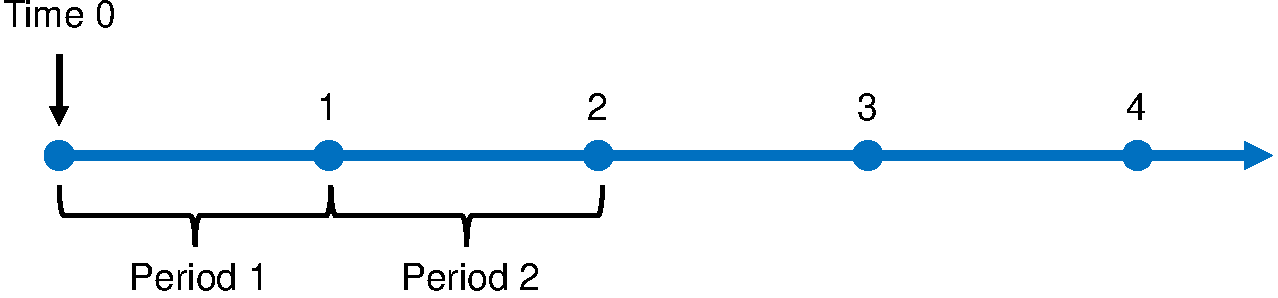
\includegraphics[width=0.6\linewidth]{figures/period_timeline.png}
\end{center}

\begin{example}[Loan Repayment Diagram]
    \$1,000 is borrowed on January 1 and repaid in 6 monthly installments
    of \$172.50 ($i=1\%$ per month). The time line's origin is the start of
    the analysis (time 0 = January 1, intervals are monthly). From the
    \textbf{borrower's} perspective: an inflow of \$1,000 at $t=0$, and
    outflows of \$172.50 at $t=1,\dots,6$. From the \textbf{bank's}
    perspective the diagram flips: an outflow of \$1,000 at $t=0$, and
    inflows of \$172.50 at $t=1,\dots,6$.
\end{example}

\begin{center}
    \begin{minipage}{0.46\linewidth}\centering
        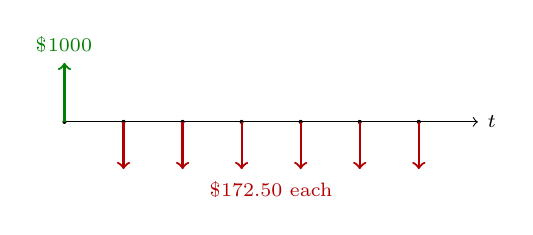
\begin{tikzpicture}[scale=0.75]
            \draw[->] (0,0) -- (7,0) node[right] {\scriptsize $t$};
            \foreach \x in {0,...,6}{\fill (\x,0) circle (1pt);}
            \draw[->,thick,green!50!black] (0,0) -- (0,1) node[above] {\scriptsize \$1000};
            \foreach \x in {1,...,6}{\draw[->,thick,red!70!black] (\x,0) -- (\x,-0.8);}
            \node[red!70!black] at (3.5,-1.15) {\scriptsize \$172.50 each};
        \end{tikzpicture}
        \\[2pt] \textit{\small Borrower}
    \end{minipage}
    \hfill
    \begin{minipage}{0.46\linewidth}\centering
        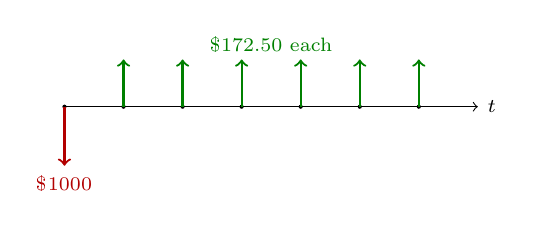
\begin{tikzpicture}[scale=0.75]
            \draw[->] (0,0) -- (7,0) node[right] {\scriptsize $t$};
            \foreach \x in {0,...,6}{\fill (\x,0) circle (1pt);}
            \draw[->,thick,red!70!black] (0,0) -- (0,-1) node[below] {\scriptsize \$1000};
            \foreach \x in {1,...,6}{\draw[->,thick,green!50!black] (\x,0) -- (\x,0.8);}
            \node[green!50!black] at (3.5,1.05) {\scriptsize \$172.50 each};
        \end{tikzpicture}
        \\[2pt] \textit{\small Bank (flipped)}
    \end{minipage}
\end{center}

\begin{example}[Reflection: Young Professional]
    Construct a cash-flow diagram for one month (assume 4 weeks per month):
    \begin{itemize}
        \item Monthly income: \$2,200 (end of each month)
        \item Rent incl.\ utilities: \$700 (end of each month)
        \item Weekly food and entertainment: \$120
        \item Telephone bill: \$40 (end of the first week of each month)
        \item Credit card purchases: \$300 (end of the second week of each month)
    \end{itemize}
    \db{Use weeks as periods and net everything at the end of each week:}
    \begin{align*}
        \text{Week 1} &: -120 - 40 = \db{-\$160}\\
        \text{Week 2} &: -120 - 300 = \db{-\$420}\\
        \text{Week 3} &: \db{-\$120}\\
        \text{Week 4} &: 2200 - 700 - 120 = \db{+\$1{,}380}
    \end{align*}
    \begin{center}
        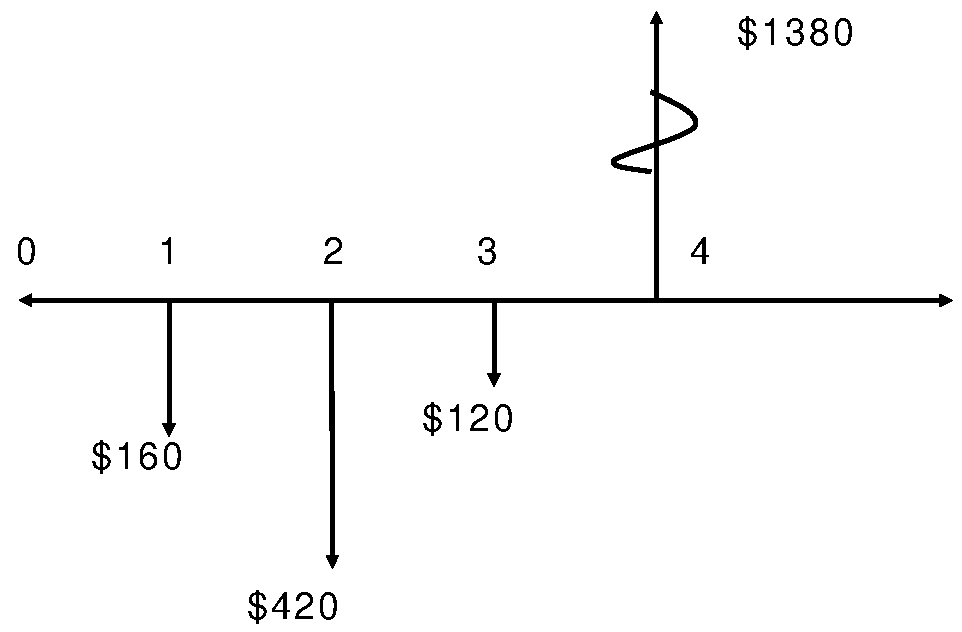
\includegraphics[width=0.5\linewidth]{figures/young_professional_cf.png}
    \end{center}
\end{example}

\topic{Categories of Regular Cash-flows}

\heading{Five Types of (Regular) Cash-flows}
\begin{enumerate}
    \item Single payments or receipts
    \item Perpetuity
    \item Annuity
    \item Arithmetic gradient
    \item Geometric gradient
\end{enumerate}

\begin{definition}[Single Payment/Receipt]
    A single cash-flow $P$ (now) or $F$ (in the future), occurring only
    once, $N$ periods apart.
\end{definition}

\begin{center}
    \begin{tikzpicture}[scale=0.8]
        \draw[->] (0,0) -- (4,0) node[right] {\scriptsize $t$};
        \fill (0,0) circle (1pt); \fill (3,0) circle (1pt);
        \node at (0,-0.35) {\scriptsize $0$};
        \node at (3,-0.35) {\scriptsize $N$};
        \draw[->,thick] (0,0) -- (0,-0.9) node[below] {\scriptsize $P$};
        \draw[->,thick] (3,0) -- (3,0.9) node[above] {\scriptsize $F$};
    \end{tikzpicture}
\end{center}

\begin{definition}[Perpetuity]
    A constant cash-flow $A$ occurring every period, forever (an
    \emph{infinite annuity}).
\end{definition}

\begin{center}
    \begin{tikzpicture}[scale=0.8]
        \draw[->] (0,0) -- (5.5,0) node[right] {\scriptsize $t$};
        \foreach \x in {1,...,5}{\fill (\x,0) circle (1pt); \draw[->,thick] (\x,0) -- (\x,0.8);}
        \node at (1,1.05) {\scriptsize $A$};
        \node at (5.8,0.4) {\scriptsize $\cdots$};
    \end{tikzpicture}
\end{center}

\begin{definition}[Annuity]
    A constant (uniform) cash-flow $A$ occurring every period, for a
    \emph{finite} number of periods $N$.
\end{definition}

\begin{center}
    \begin{tikzpicture}[scale=0.8]
        \draw[->] (0,0) -- (5,0) node[right] {\scriptsize $t$};
        \foreach \x in {1,...,4}{\fill (\x,0) circle (1pt); \draw[->,thick] (\x,0) -- (\x,0.8);}
        \node at (1,1.05) {\scriptsize $A$};
        \node at (4,-0.35) {\scriptsize $N$};
    \end{tikzpicture}
\end{center}

\begin{definition}[Arithmetic Gradient]
    A cash-flow that grows (or shrinks) by the same \emph{amount} $G$
    each period, starting from a base $A'$ at $t=1$:
    \[A',\ A'+G,\ A'+2G,\ \dots,\ A'+(N-1)G.\]
    It splits into an annuity of $A'$ (red, below) plus a pure gradient
    $G, 2G, \dots$ on top (black).
\end{definition}

\begin{center}
    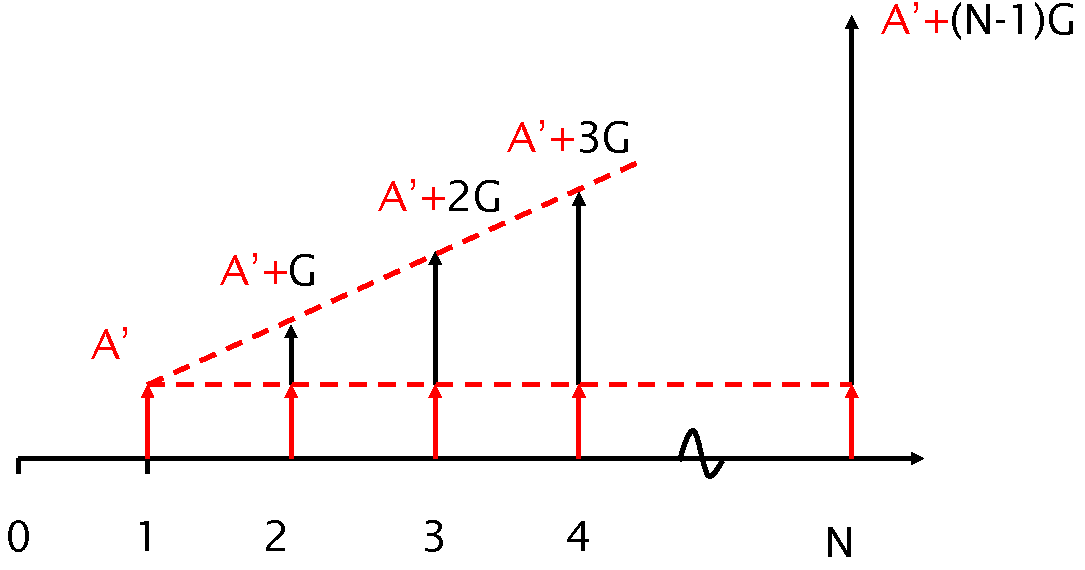
\includegraphics[width=0.55\linewidth]{figures/arithmetic_gradient.png}
\end{center}

\begin{definition}[Geometric Gradient]
    A cash-flow that grows (or shrinks) by the same \emph{percentage} $g$
    each period, starting from $A$ at $t=1$:
    \[A,\ A(1+g),\ A(1+g)^2,\ \dots,\ A(1+g)^{N-1}.\]
    There must be a cash-flow at the end of period 1, otherwise there is
    nothing for the percentage to grow from.
\end{definition}

\begin{center}
    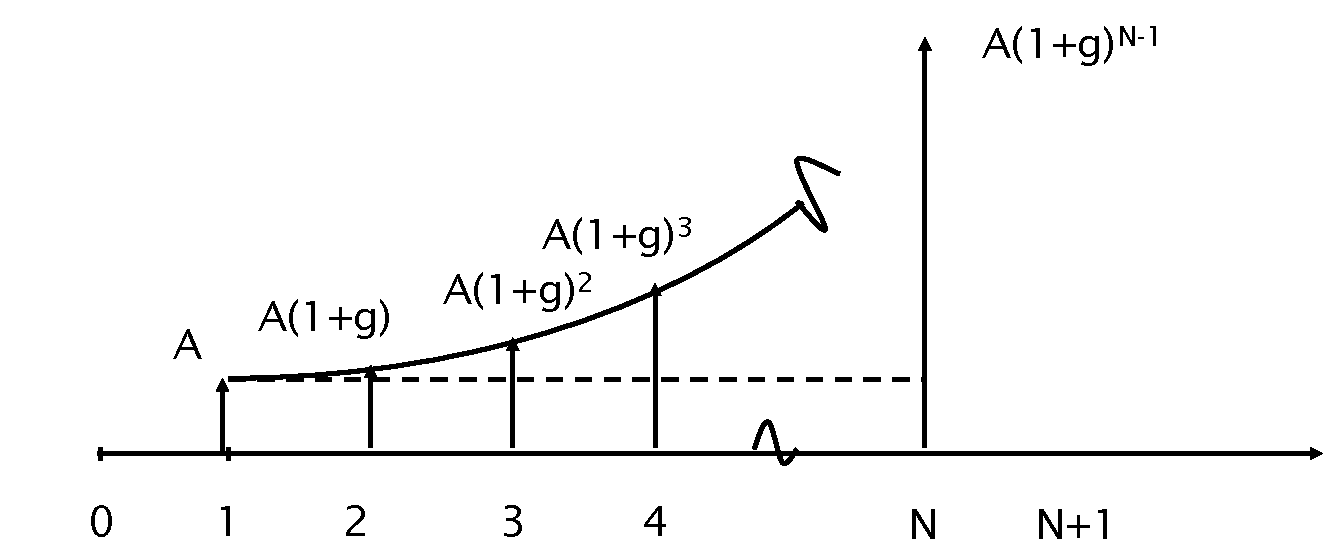
\includegraphics[width=0.6\linewidth]{figures/geometric_gradient.png}
\end{center}

\topic{Cash-flow Equivalence}

\heading{Three Concepts of Equivalence}
\begin{itemize}
    \item \rb{Mathematical}: consequence of the mathematical relationship between time and money
    \item \rb{Market}: consequence of the ability to exchange one cash-flow for another at zero cost
    \item \rb{Decisional}: due to indifference on the part of the decision maker among available choices
\end{itemize}

\begin{definition}[Mathematical Equivalence]
    A consequence of the mathematical relationship between time and
    money. Two cash-flows $P_t$ (at time $t$) and $F_{t+N}$ (at time
    $t+N$) are equivalent at rate $i$ if
    \[F_{t+N} = P_t(1+i)^N \iff P_t = \frac{F_{t+N}}{(1+i)^N}.\]
    If a further cash-flow $F_{t+N+M}$ is also equivalent to $P_t$, then
    \[F_{t+N+M} = P_t(1+i)^{N+M} = F_{t+N}(1+i)^M \iff P_t = \frac{F_{t+N+M}}{(1+i)^{N+M}},\]
    i.e.\ equivalent amounts compound/discount consistently with each other.
\end{definition}

\begin{center}
    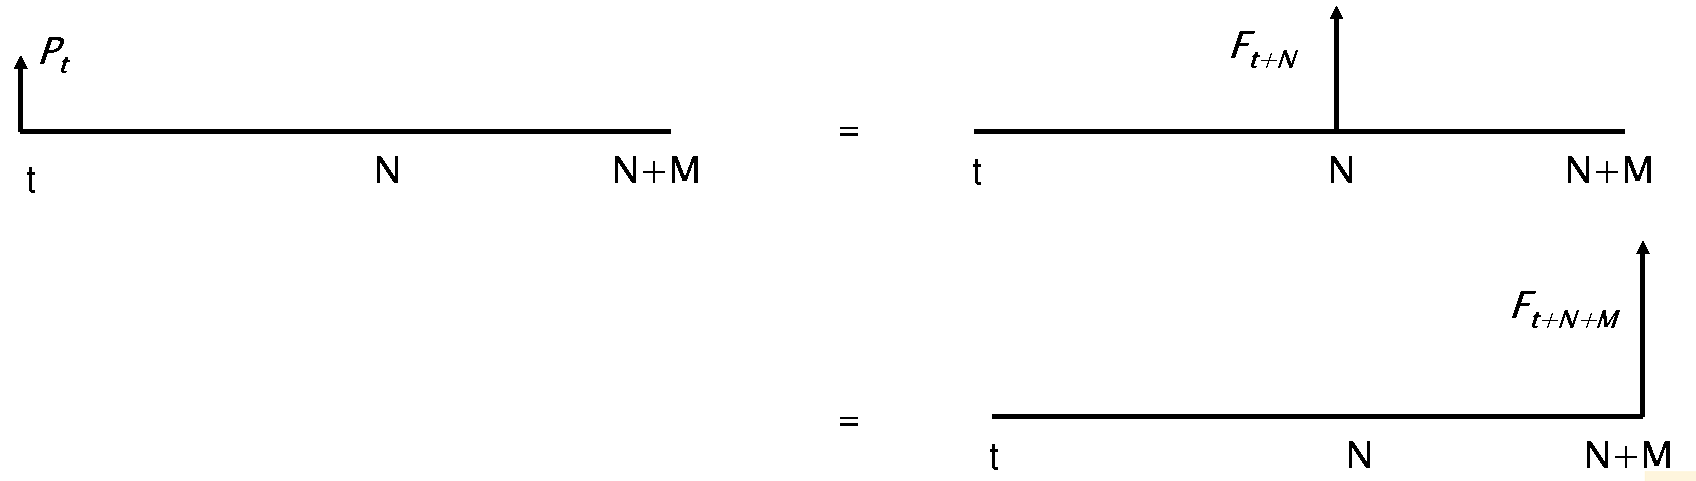
\includegraphics[width=0.75\linewidth]{figures/math_equivalence.png}
\end{center}

\begin{definition}[Market Equivalence]
    A consequence of being able to exchange one cash-flow for another at
    \emph{zero cost}. Exchanging a future cash-flow for a present one is
    \textbf{borrowing}; giving up a present cash-flow for a future one is
    \textbf{lending/investing}. In real markets, borrowing and lending
    rates usually differ.
\end{definition}

\begin{example}[T-bill Market Equivalence]
    A T-bill is a short-term government debt obligation (maturity $\le 1$
    year), usually sold in \$1,000 denominations. A \$1,000 T-bill
    maturing in 6 months currently sells for \$990.10: some holders are
    willing to sell at this price and others to buy. The market has agreed
    this corresponds to an interest rate of 1\% over 6 months. Confirm:
    \[i = \frac{1000}{990.10} - 1 = \db{0.0100 = 1\%}\]
\end{example}

\begin{definition}[Decisional Equivalence]
    Two cash-flows $P_t$ and $F_{t+N}$ are equivalent for a decision
    maker if they are \emph{indifferent} between them. Here the interest
    rate is not known a priori --- instead, an \rb{implied} rate can be
    backed out from the decision that the two are equivalent.
\end{definition}

\begin{example}[Implied Interest Rate]
    A manufacturer needs 1,000~kg of aluminium on August 15 but is
    offered 1,100~kg on August 22 instead (same price, paid at the end
    of August).
    \[i = \frac{1100}{1000} - 1 = \db{10\% \text{ for one week}}\]
    \db{The real question is whether the extra 100~kg is worth the cost of the one-week delay to this decision maker. If they are indifferent, 10\%/week is their implied rate.}
\end{example}

\begin{remark}
    Financial analysis uses \textbf{mathematical} and \textbf{market}
    equivalence to decide whether to invest or not invest.
\end{remark}

\topic{Cash-flow Factors}

\begin{remark}[Standing Assumptions]
    Unless otherwise noted:
    \begin{enumerate}
        \item Interest compounds once per period.
        \item Cash-flow occurs at the end of the period.
        \item Time 0 is period 0, i.e.\ the start of period 1.
        \item All periods are the same length.
    \end{enumerate}
\end{remark}

\begin{definition}[Cash-flow Symbols]
    $P$: a single cash-flow today. $F$: a single cash-flow in the
    future. $A$: a finite series of equal cash-flows at regular
    intervals (annuity). $G$: a cash-flow growing by a fixed
    \emph{amount} each period (arithmetic gradient) or fixed
    \emph{percentage} $g$ each period (geometric gradient, ``Geom'').
\end{definition}

\begin{definition}[Factor Notation]
    $(X/Y,i,N)$ converts a cash-flow of type $Y$ into the equivalent
    amount of type $X$ at rate $i$ over $N$ periods: $X = Y\cdot
    (X/Y,i,N)$. E.g.\ $F = P(F/P,i,N)$; for geometric gradients,
    $P = G(P/\text{Geom},i,g,N)$.
\end{definition}

\begin{center}
    \begin{tabular}{ll}
        \toprule
        Factor & Name \\
        \midrule
        $(F/P,i,N)$ & Compound amount factor \\
        $(P/F,i,N)$ & Present worth factor \\
        $(A/F,i,N)$ & Sinking fund factor \\
        $(F/A,i,N)$ & Series compound amount factor \\
        $(A/P,i,N)$ & Capital recovery factor \\
        $(P/A,i,N)$ & Series present worth factor \\
        $(P/G,i,N)$ & Arithmetic gradient to present worth \\
        $(P/\text{Geom},i,g,N)$ & Geometric gradient to present worth \\
        \bottomrule
    \end{tabular}
\end{center}

\begin{remark}[Relating Factors]
    Factors invert: since $P = A(P/A,i,N)$,
    \[A = \frac{P}{(P/A,i,N)} = P(A/P,i,N) \quad\Rightarrow\quad (A/P,i,N) = \frac{1}{(P/A,i,N)}.\]
    The same trick relates any pair of factors.
\end{remark}

\begin{definition}[Single-Payment Factors]
    $P$ and $F$ are related by compounding one period at a time,
    $F_n = F_{n-1}(1+i)$, so $F = P(1+i)^N$:
    \[(F/P,i,N) = (1+i)^N, \qquad (P/F,i,N) = (1+i)^{-N}.\]
\end{definition}

\begin{center}
    \begin{tikzpicture}[scale=1]
        \draw[->] (0,0) -- (4.6,0) node[right] {\scriptsize $N$};
        \draw[->] (0,0) -- (0,2.3) node[above] {\scriptsize $(P/F,i,N)$};
        \foreach \x/\lbl in {0/0,1/2,2/4,3/6,4/8}{
            \draw (\x,0.05) -- (\x,-0.05);
            \node[below] at (\x,-0.08) {\scriptsize \lbl};
        }
        \node[left] at (0,2) {\scriptsize $1.0$};
        \draw[thick,blue!60!black] plot coordinates
            {(0,2)(0.5,1.818)(1,1.652)(1.5,1.502)(2,1.366)(2.5,1.242)(3,1.128)(3.5,1.026)(4,0.934)};
    \end{tikzpicture}
    \\[2pt] \textit{\small $(1+i)^{-N}$ decays toward $0$ as $N$ grows (shown for $i=10\%$)}
\end{center}

\begin{example}[F/P]
    If you had \$2,000 now and invested it at 10\%, how much would it be worth in 8 years?
    \[F = 2000(F/P,10\%,8) = 2000(1.10)^8 = 2000(2.1436) = \db{\$4{,}287.18}\]
\end{example}

\begin{example}[P/F: Solving for $i$]
    You invest \$1,100 today and expect \$2,000 in 8 years. What is the interest rate?
    \[1100 = 2000(P/F,i,8) \;\Rightarrow\; (1+i)^8 = \frac{2000}{1100} = 1.8182 \;\Rightarrow\; i = 1.8182^{1/8} - 1 = \db{7.76\%}\]
\end{example}

\begin{example}[Present Value of a Perpetuity]
    Invest \$100 and get paid 5\% interest in cash every year, forever.
    Each year the \$5 of interest is paid out, so the balance never changes:
    \begin{center}
    \begin{tabular}{cccc}
        \toprule
        Year & Interest & Cash-flow & Amount in bank at year end \\
        \midrule
        0 & --- & $-100$ & 100 \\
        1 & 5 & $+5$ & 100 \\
        2 & 5 & $+5$ & 100 \\
        3 & 5 & $+5$ & 100 \\
        $\vdots$ & $\vdots$ & $\vdots$ & $\vdots$ \\
        \bottomrule
    \end{tabular}
    \end{center}
    \db{So \$100 today is equivalent to \$5/year forever, i.e.\ $P = A/i = 5/0.05 = 100$.} In general, a constant amount $A$ paid forever has a finite present value:
    \[P = \frac{A}{1+i}+\frac{A}{(1+i)^2}+\cdots = \boxed{\frac{A}{i}}.\]
\end{example}

\begin{definition}[Present Worth of an Annuity]
    An annuity of $A$ for $N$ periods is a perpetuity starting now minus a
    perpetuity starting at $N$ (worth $A/i$ at time $N$, discounted back):
    \[(P/A,i,N) = \frac{1}{i}-\frac{1}{i(1+i)^N}
    = \frac{(1+i)^N - 1}{i(1+i)^N}.\]
    Combining with $(F/P)$ and inverting gives the rest of the uniform-series factors:
    \[(F/A,i,N) = \frac{(1+i)^N-1}{i}, \qquad (A/F,i,N) = \frac{i}{(1+i)^N-1}, \qquad (A/P,i,N) = \frac{i(1+i)^N}{(1+i)^N-1}.\]
\end{definition}

\begin{definition}[Present Worth of an Arithmetic Gradient]
    For a gradient contributing $G,2G,\dots,(N-1)G$ starting at $t=2$
    (no cash-flow at $t=0$ or $t=1$):
    \[(P/G,i,N) = \frac{1}{i^2}\left(1-\frac{1+iN}{(1+i)^N}\right).\]
    A series with initial amount $A$ growing by $G$ each period splits
    into an annuity plus a gradient:
    \[P = A(P/A,i,N) + G(P/G,i,N).\]
\end{definition}

\begin{center}
    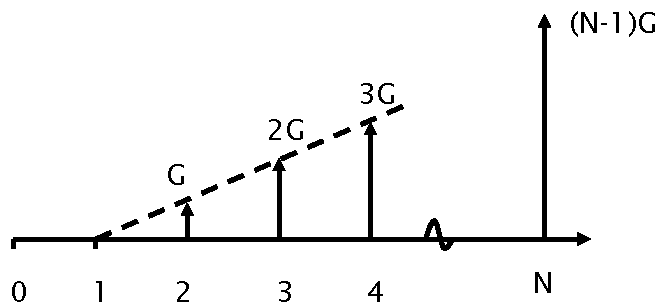
\includegraphics[width=0.45\linewidth]{figures/gradient_G_only.png}
    \\[2pt] \textit{\small The pure gradient: nothing at $t=0,1$; $G$ at $t=2$, \dots, $(N-1)G$ at $t=N$}
\end{center}

\begin{remark}[Sign Combinations for Arithmetic Gradients]
    Besides $G=0$, four cases: $A>0,\,G>0$ (positive, increasing);
    $A>0,\,G<0$ (positive, decreasing); $A<0,\,G>0$ (negative, becoming
    less so); $A<0,\,G<0$ (negative, becoming more so).
\end{remark}

\begin{definition}[Present Worth of a Geometric Gradient]
    For a series $A,\,A(1+g),\,A(1+g)^2,\dots$ starting at $t=1$:
    \[(P/\text{Geom},i,g,N) = \frac{1-\left(\frac{1+g}{1+i}\right)^N}{i-g}
    = \frac{(P/A,i_o,N)}{1+g}, \qquad i_o = \frac{1+i}{1+g}-1.\]
\end{definition}

\begin{remark}
    Regardless of the pattern, present value always follows from
    discounting each cash-flow individually and summing. Each period a
    cash-flow is moved forward, multiply by $(1+i)$; each period back,
    divide by $(1+i)$:
    \[\boxed{P = \frac{F_1}{1+i}+\frac{F_2}{(1+i)^2}+\cdots = \sum_t \frac{F_t}{(1+i)^t}.}\]
\end{remark}

\heading{Factor Table ($i = 10\%$)}
\begin{center}
    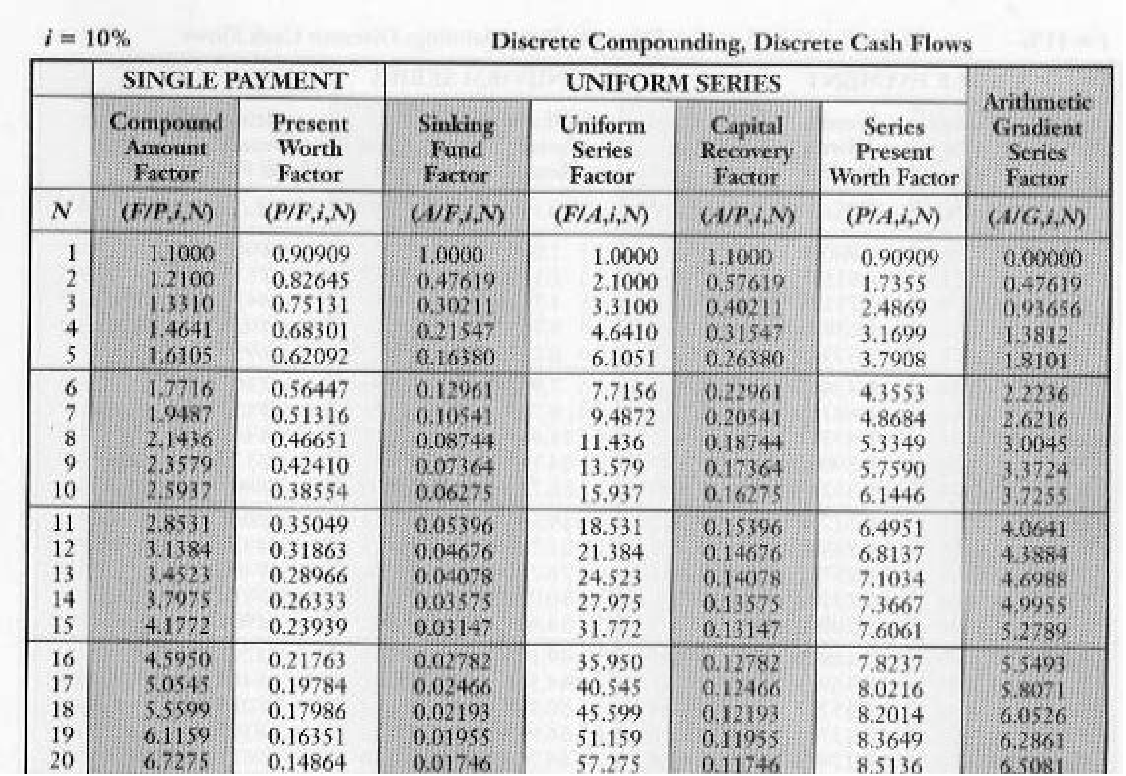
\includegraphics[width=0.75\linewidth]{figures/factor_table_10pct.png}
\end{center}

\begin{example}[Reflection: Lump Sums vs.\ Annuity]
    Which option do you prefer if interest is 8\%?
    (a) \$20,000 now and \$50,000 at the end of 10 years, or
    (b) ten equal annual receipts of \$7,000?
    \begin{align*}
        P_a &= 20{,}000 + 50{,}000(P/F,8\%,10) = 20{,}000 + 50{,}000(0.46319) = \db{\$43{,}160}\\
        P_b &= 7{,}000(P/A,8\%,10) = 7{,}000(6.7101) = \db{\$46{,}971}
    \end{align*}
    \db{Prefer (b): it has the higher present value.}
\end{example}

\begin{example}[Reflection: Annuity at a Lower Rate]
    \$1/year for 5 years has a present value of \$3.7908 at 10\%. Which is a likely value at 9\%?
    (a) 3.8897 \quad (b) 5.0000 \quad (c) 3.7908 \quad (d) 2.3262
    \\\db{(a) 3.8897. A lower rate discounts less, so PV rises above 3.7908, but it must stay below the undiscounted total of \$5. Check: $(P/A,9\%,5) = 3.8897$.}
\end{example}

\topic{Worked Examples}

\begin{example}[Investment Decision]
    An investor can buy a tract of land that will be worth \$10,000 in
    six years. If the rate of return on land is 8\%, how much should the
    investor be willing to pay now?
    \[P = 10{,}000(P/F,8\%,6) = \frac{10{,}000}{(1.08)^6} = \db{\$6{,}301.70}\]
\end{example}

\begin{example}[The Magic of Compounding]
    At age 20 you save and invest \$1.00 each day (\$365/year) until age 80,
    at 10\% annual interest.
    \[F = 365(F/A,10\%,60) = 365\cdot\frac{(1.10)^{60}-1}{0.10} \approx \db{\$1{,}107{,}708}\]
    \db{You become a millionaire.}
\end{example}

\begin{example}[F and P with Subperiod Compounding]
    How much is accumulated over 5 years in each savings plan?
    \begin{itemize}
        \item \$2,000 today at 10\% compounded semi-annually: $i_s = 5\%$, $N = 10$
        \[F = 2000(1.05)^{10} = \db{\$3{,}257.79}\]
        \item \$1,000 today at 12\% compounded monthly: $i_s = 1\%$, $N = 60$
        \[F = 1000(1.01)^{60} = \db{\$1{,}816.70}\]
    \end{itemize}
    How much must you invest today to get \$2,000 in 5 years at 8\% compounded quarterly? $i_s = 2\%$, $N = 20$:
    \[P = 2000(P/F,2\%,20) = \frac{2000}{(1.02)^{20}} = \db{\$1{,}345.94}\]
\end{example}

\begin{example}[Mortgage/Amortization]
    A \$300,000 mortgage at a nominal 9\% (mortgages are quoted with
    semi-annual compounding) is amortized over 15 years. What is the monthly payment?
    \\\db{Semi-annual rate $= 4.5\%$. The equivalent monthly rate satisfies $(1+i_m)^6 = 1.045$:}
    \[i_m = 1.045^{1/6} - 1 = 0.7363\%, \qquad N = 15 \times 12 = 180\]
    \[A = 300{,}000(A/P,0.7363\%,180) = \db{\$3{,}013.56 \text{ per month}}\]
    \db{That is about \$36,163/year, over 70\% of a \$50k starting salary (before tax), so it doesn't fit the budget.}
\end{example}

\begin{example}[Sinking Fund]
    A ``targeted'' $F$ calculation: save up to pay a future expenditure
    (e.g.\ replacing a machine). A roof must be replaced in 10 years for
    an estimated \$28,000. What equal end-of-year deposits at 8\% are needed?
    \[A = 28{,}000(A/F,8\%,10) = 28{,}000\cdot\frac{0.08}{(1.08)^{10}-1} = \db{\$1{,}932.83 \text{ per year}}\]
\end{example}

\begin{example}[Retirement Planning]
    You are 20 and want \$1,000,000 at retirement at 65 (45 years). What
    equal end-of-year savings are needed at 7\%? At 10\%?
    \begin{align*}
        A_{7\%} &= 1{,}000{,}000(A/F,7\%,45) = \db{\$3{,}499.57 \text{ per year}}\\
        A_{10\%} &= 1{,}000{,}000(A/F,10\%,45) = \db{\$1{,}391.00 \text{ per year}}
    \end{align*}
\end{example}

\begin{example}[Uneven Annuity Segments]
    Claudia wants to deposit $P$ now so that she can withdraw \$2,000/year
    for 5 years and then \$3,000/year for the next 3 years, at 8\%.
    Discount the second annuity back to $t=5$, then to $t=0$:
    \begin{align*}
        P &= 2{,}000(P/A,8\%,5) + 3{,}000(P/A,8\%,3)(P/F,8\%,5)\\
        &= 2{,}000(3.9927) + 3{,}000(2.5771)(0.68058)\\
        &= 7{,}985.42 + 5{,}261.79 = \db{\$13{,}247.21}
    \end{align*}
    \begin{center}
    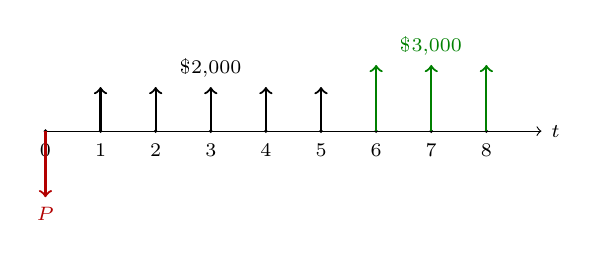
\begin{tikzpicture}[scale=0.7]
        \draw[->] (0,0) -- (9,0) node[right] {\scriptsize $t$};
        \foreach \x in {0,...,8}{\fill (\x,0) circle (1pt); \node[below] at (\x,-0.05) {\scriptsize \x};}
        \draw[->,thick,red!70!black] (0,0) -- (0,-1.2) node[below] {\scriptsize $P$};
        \foreach \x in {1,...,5}{\draw[->,thick] (\x,0) -- (\x,0.8);}
        \foreach \x in {6,7,8}{\draw[->,thick,green!50!black] (\x,0) -- (\x,1.2);}
        \node[above] at (3,0.8) {\scriptsize \$2,000};
        \node[above,green!50!black] at (7,1.2) {\scriptsize \$3,000};
    \end{tikzpicture}
    \end{center}
\end{example}

\begin{example}[Present Value with an Arithmetic Gradient: Investment]
    An investment of \$400,000 pays benefits of 20\% (\$80,000) in year 1,
    with an additional \$15,000 added to each previous year's benefit, for
    5 years. At a 10\% discount rate, is it worth it?
    \begin{align*}
        P &= -400{,}000 + 80{,}000(P/A,10\%,5) + 15{,}000(P/G,10\%,5)\\
        &= -400{,}000 + 80{,}000(3.7908) + 15{,}000(6.8618)\\
        &= -400{,}000 + 406{,}190 = \db{+\$6{,}190}
    \end{align*}
    \db{Barely worth it: the benefits' PV just exceeds the \$400,000 cost.}
\end{example}

\begin{example}[Present Value with an Arithmetic Gradient: Maintenance]
    A machine costs \$155 to maintain this year, with maintenance
    costing \$35 more each subsequent year, over an 8-year life at 6\%.
    How much must be invested now to cover maintenance, and what is the
    Equivalent Annual Cost (EAC)?
    \begin{align*}
        P &= 155(P/A,6\%,8) + 35(P/G,6\%,8) = 155(6.2098) + 35(19.8416) = \db{\$1{,}656.97}\\
        \text{EAC} &= P(A/P,6\%,8) = 1{,}656.97(0.16104) = \db{\$266.83 \text{ per year}}
    \end{align*}
    With a \$1,000 overhaul at the start ($t=0$):
    \[\text{EAC} = (1{,}656.97 + 1{,}000)(A/P,6\%,8) = \db{\$427.87 \text{ per year}}\]
\end{example}

\begin{example}[Future Value with Periodic Dividends]
    \$100,000 is loaned at 15\% (interest compounded annually, not paid out),
    with a \$5,000 dividend at the end of every third year for 15 years,
    reinvested at 15\%. How much do you have at the end?
    \\\db{Principal: $100{,}000(1.15)^{15} = \$813{,}706$. The dividends are an
    annuity with 3-year periods ($N=5$), so use the 3-year effective rate
    $i_3 = (1.15)^3 - 1 = 52.09\%$:}
    \begin{align*}
        F &= 100{,}000(F/P,15\%,15) + 5{,}000(F/A,52.09\%,5)\\
        &= 813{,}706 + 68{,}510 = \db{\$882{,}216}
    \end{align*}
\end{example}

\begin{example}[A Business Example]
    Over 3 years a small business has:
    \begin{itemize}
        \item sales of \$240k, \$360k, \$480k per year, received in equal monthly amounts (\$20k, \$30k, \$40k/month)
        \item investments of \$15k/quarter in year 1, \$20k/quarter in year 2, \$25k/quarter in year 3
        \item an initial investment of \$100k, and a salvage value of \$70k after 3 years
    \end{itemize}
    What is the PV at 12\%, analysed on monthly cash-flows?
    \\\db{Monthly rate $i = 12\%/12 = 1\%$. Each year's sales are a 12-month annuity shifted to the start of its year; quarterly investments fall at months $3, 6, \dots, 36$:}
    \begin{align*}
        P ={}& -100{,}000 + \big[20{,}000 + 30{,}000(P/F,1\%,12) + 40{,}000(P/F,1\%,24)\big](P/A,1\%,12)\\
        & - \sum_{q=1}^{12} Q_q (P/F,1\%,3q) + 70{,}000(P/F,1\%,36)\\
        \approx{}& \db{\$633{,}463}
    \end{align*}
    \db{where $Q_q$ is \$15k, \$20k or \$25k depending on the year.}
\end{example}

% !TeX root = ../main.tex

% Edit this title for each week's entry.
\section{Week 3 - Financial Instruments}

\topic{Mortgages}

\begin{definition}[Mortgage]
    A loan secured by \textbf{real property}: you borrow money and use the
    property as collateral. From French law, ``death contract'' (\emph{mort-}
    = death): the pledge ends when the obligation is fulfilled.
\end{definition}

\heading{Importance of Mortgages}
\begin{itemize}
    \item The most common way to finance a home: new purchases with a mortgage outnumber those without by a factor of 6 (CMHC)
    \item Mortgages are by far the largest share of Canadian household debt
\end{itemize}
\begin{center}
    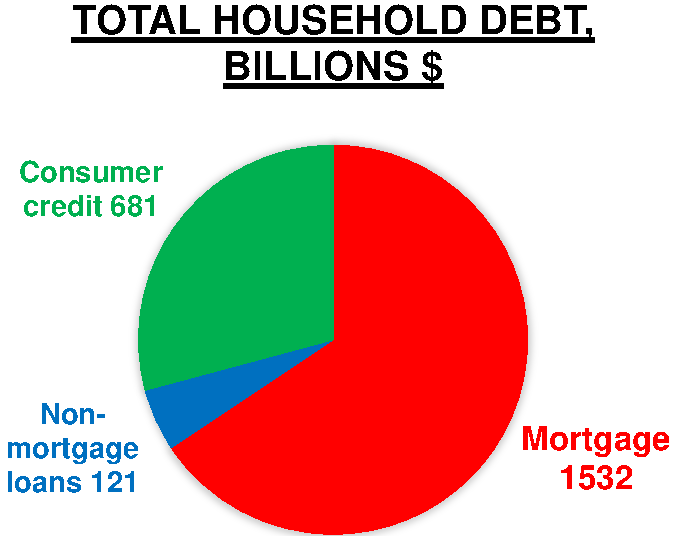
\includegraphics[width=0.35\linewidth]{figures/household_debt_pie.png}
    \\[2pt] \textit{\small Total household debt, billions \$ (Statistics Canada)}
\end{center}

\heading{Mortgage Terminology}
Buying a \$500,000 house:
\begin{itemize}
    \item \rb{Principal}: the amount you borrow, up to some fraction of the price (e.g.\ 80\% $\Rightarrow$ \$400,000)
    \item \rb{Down payment}: the rest, which you pay yourself (\$100,000)
    \item \rb{Loan-to-value ratio (LTV)}: mortgage loan / value of house $= 400{,}000/500{,}000 = 0.8$
    \item \rb{Mortgage rate}: the interest rate the bank charges on the principal (e.g.\ 5\%/year)
    \item \rb{Amortization period}: the agreed time horizon for full repayment (e.g.\ 25 years)
    \item \rb{Term}: the shorter period over which the agreed rate is fixed (e.g.\ 5 years). After the term ends, the rate is renegotiated and the payments may change
\end{itemize}

\begin{remark}
    Payments are calculated based on the \textbf{amortization period},
    \textbf{not} the term! Canadian mortgage rates are quoted as nominal
    annual rates with \textbf{semi-annual compounding}, so convert to the
    equivalent monthly rate before using $(A/P,i,N)$.
\end{remark}

\begin{example}[Mortgage Payments Across Terms]
    A \$500,000 home with a 20\% down payment. The mortgage rate is 5\%,
    with a 5-year term and a 25-year amortization period.
    \begin{enumerate}[label = \alph*)]
        \item What is the monthly payment during this term?
        \\\db{Principal $P = 0.8(500{,}000) = \$400{,}000$. Semi-annual rate $2.5\%$, so the monthly rate satisfies $(1+i_m)^6 = 1.025$:}
        \[i_m = 1.025^{1/6} - 1 = 0.41239\%, \qquad N = 25 \times 12 = 300\]
        \[A = 400{,}000(A/P,0.41239\%,300) = \db{\$2{,}326.42 \text{ per month}}\]
        \item After the term, the new mortgage rate is 6\%. What is the new monthly payment?
        \\\db{The amount still owed after 60 payments is the PV of the 240 remaining payments at the old rate:}
        \[B_{60} = 2{,}326.42(P/A,0.41239\%,240) = \$354{,}030\]
        \db{Re-amortize this over the remaining 20 years at the new rate, $i_m' = 1.03^{1/6} - 1 = 0.49386\%$:}
        \[A' = 354{,}030(A/P,0.49386\%,240) = \db{\$2{,}521.36 \text{ per month}}\]
    \end{enumerate}
\end{example}

\begin{center}
    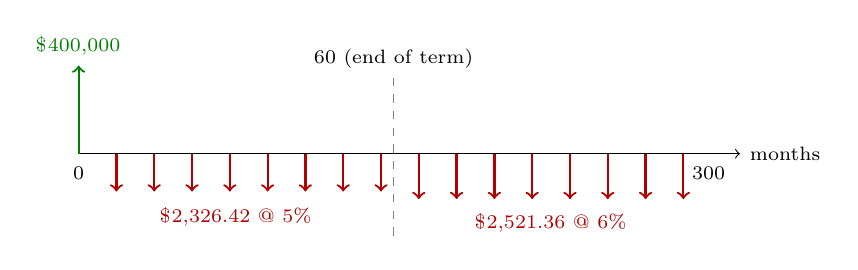
\begin{tikzpicture}[scale=0.8]
        \draw[->] (0,0) -- (10.5,0) node[right] {\scriptsize months};
        \draw[->,thick,green!50!black] (0,0) -- (0,1.4) node[above] {\scriptsize \$400,000};
        \foreach \x in {0.6,1.2,...,4.9}{\draw[->,thick,red!70!black] (\x,0) -- (\x,-0.6);}
        \foreach \x in {5.4,6.0,...,9.9}{\draw[->,thick,red!70!black] (\x,0) -- (\x,-0.72);}
        \draw[dashed,gray] (5,-1.3) -- (5,1.2);
        \node[below] at (0,-0.05) {\scriptsize 0};
        \node[above] at (5,1.2) {\scriptsize 60 (end of term)};
        \node[below] at (10,-0.05) {\scriptsize 300};
        \node[red!70!black] at (2.5,-1.0) {\scriptsize \$2,326.42 @ 5\%};
        \node[red!70!black] at (7.5,-1.1) {\scriptsize \$2,521.36 @ 6\%};
    \end{tikzpicture}
    \\[2pt] \textit{\small Borrower's view: payments step up at the renewal}
\end{center}

\heading{Some Canadian Mortgage Rules}
\begin{itemize}
    \item Since 2012, amortization periods of up to 25 years are allowed
    \item For 25-year amortization, the down payment must be at least 20\%
    \item For shorter amortization periods, the down payment may be smaller ($<20\%$), but \b{mortgage insurance} is required
    \item Real-life mortgages can be more complicated: rates can be variable within a term, you can pay the mortgage down faster, \dots
\end{itemize}

\heading{Summary}
\begin{enumerate}
    \item Mortgages are loans backed by real property (the most common way to finance a home)
    \item Payments are calculated from the principal, mortgage rate, and \b{amortization period}
    \item At the end of each term, the next payments are set by the \b{amount still owed}, the \b{new rate}, and the \b{remaining amortization period}
\end{enumerate}

\topic{Bonds}

\begin{definition}[Bond]
    A financial instrument issued by firms and governments (federal,
    provincial, municipal) to raise funds for projects. It is a special form
    of loan, usually long-term (up to 30 years). The issuer (the borrower)
    promises to pay:
    \begin{itemize}
        \item a stated amount at specified intervals for a defined period: the \rb{coupon payments}
        \item a final amount at a specific date: the \rb{face value}
    \end{itemize}
    Bonds are usually tradeable at any time.
\end{definition}

\heading{Reading a Bond (Ontario Hydro)}
\begin{itemize}
    \item \rb{Face value}: the amount paid at maturity (\$1,000)
    \item \rb{Maturity date}: when the face value is paid (January 6, 2004)
    \item \rb{Coupon rate}: the (nominal annual) rate used to calculate coupon payments ($9\tfrac14\%$)
    \item \rb{Coupon frequency}: how often coupons are paid (January 6 and July 6, i.e.\ semi-annually)
\end{itemize}
\begin{center}
    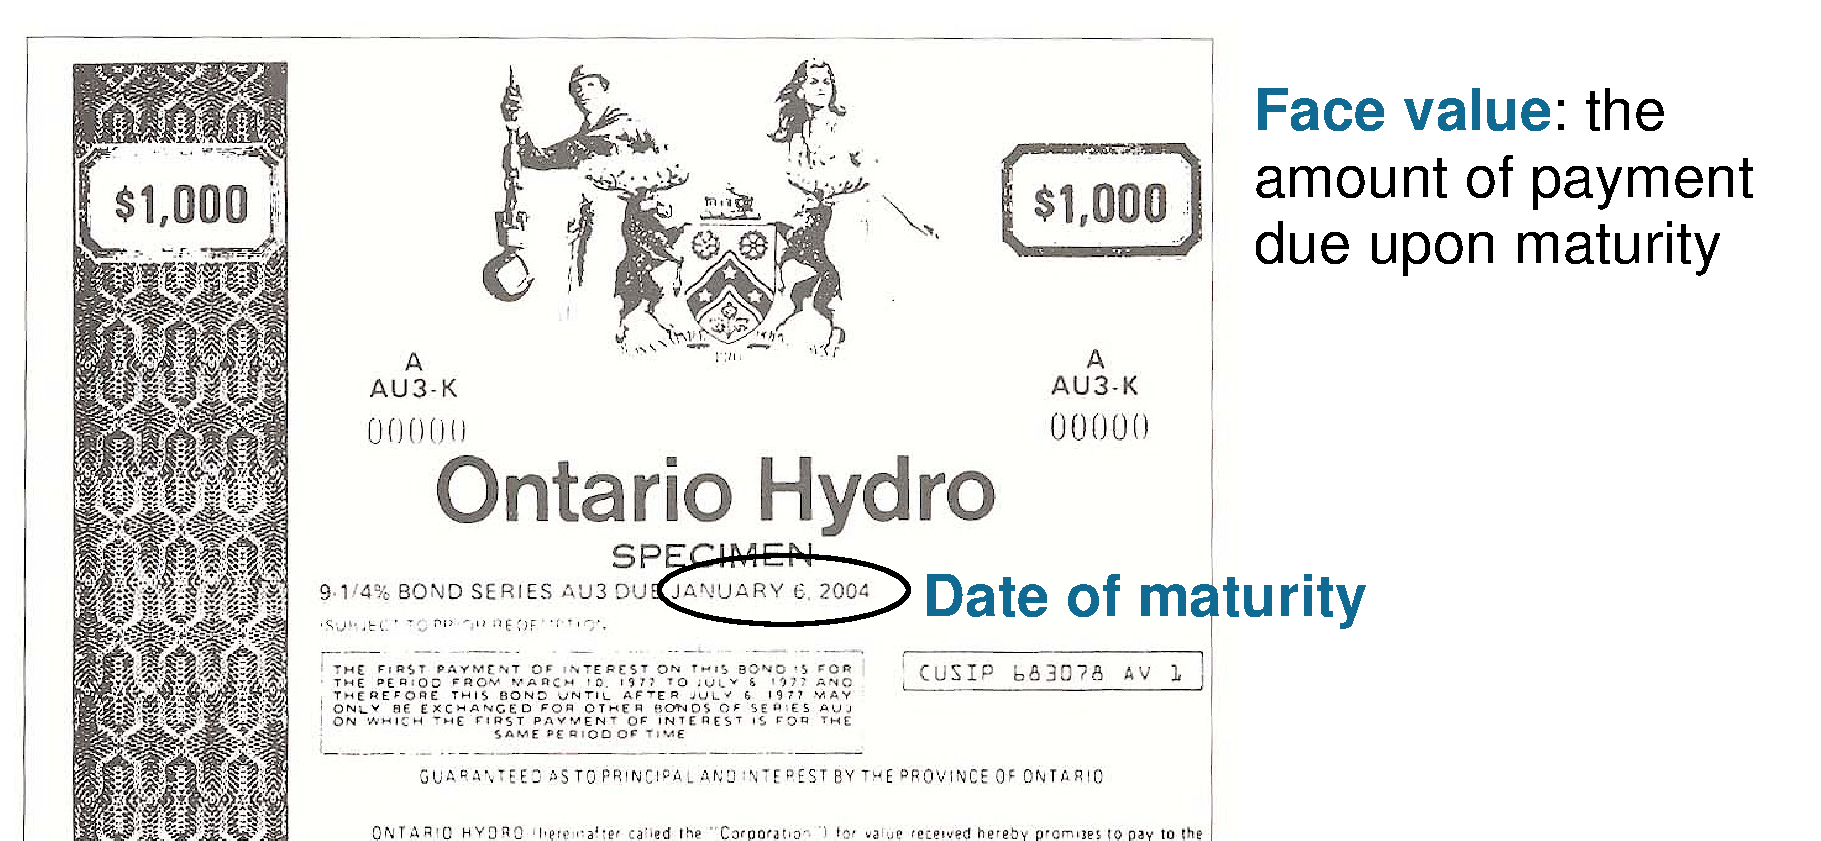
\includegraphics[width=0.62\linewidth]{figures/bond_face_annotated.png}
    \\[4pt]
    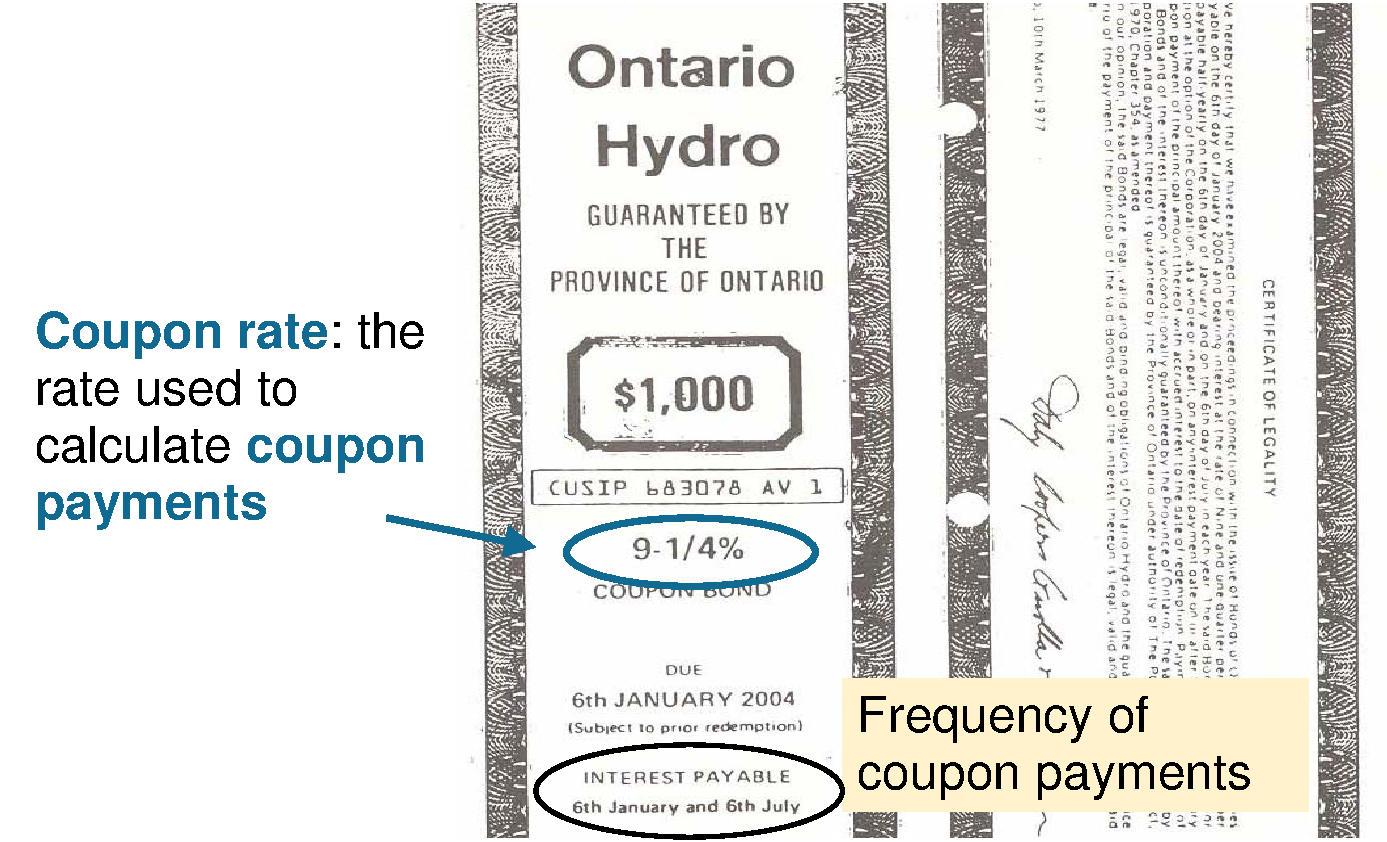
\includegraphics[width=0.5\linewidth]{figures/bond_back_annotated.png}
    \hspace{1em}
    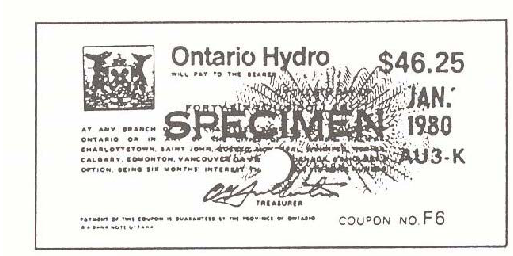
\includegraphics[width=0.3\linewidth]{figures/bond_coupon.png}
\end{center}
\db{Each semi-annual coupon $= 1000 \times 9.25\% / 2 = \$46.25$, matching the coupon shown.}

\heading{Bond Cash-flow Diagram}
From the bondholder's view: pay the price $P$ now, receive coupon $C$ every
period for $N$ periods, plus the face value $F$ at maturity.
\begin{center}
    \begin{tikzpicture}[scale=0.8]
        \draw[->] (0,0) -- (8.5,0) node[right] {\scriptsize $t$};
        \foreach \x in {1,...,7}{\draw[->,thick,green!50!black] (\x,0) -- (\x,0.6);}
        \draw[->,thick,green!50!black] (7,0.6) -- (7,2) node[above] {\scriptsize $F$};
        \node[green!50!black] at (4,0.9) {\scriptsize $C$ each period};
        \draw[->,thick,red!70!black] (0,0) -- (0,-1.2) node[below] {\scriptsize price $P$};
        \node[below] at (7,-0.05) {\scriptsize $N$};
    \end{tikzpicture}
\end{center}
\[\boxed{P = C(P/A,i,N) + F(P/F,i,N)}\]
where $i$ is the yield per coupon period.

\begin{example}[How Much Is This Bond Worth?]
    Ontario Hydro will pay you \$1,000 in 10 years, plus coupons at 9.25\%
    paid every 6 months. If the bank pays 10\% interest, what amount must be
    deposited now to produce the same cash-flows?
    \\\db{$C = \$46.25$, $N = 20$ half-years, $i = 10\%/2 = 5\%$ per half-year:}
    \begin{align*}
        P &= 46.25(P/A,5\%,20) + 1000(P/F,5\%,20)\\
        &= 46.25(12.4622) + 1000(0.37689) = \db{\$953.27}
    \end{align*}
    Would you be willing to pay \$953?
    \\\db{Only if the bond were as safe as the bank. Ontario Hydro might default, so you should demand a lower price.}
\end{example}

\begin{definition}[Yield]
    Risk == reward: the buyer must be compensated for the risk of default by
    paying a \textbf{lower} price. The \rb{yield} is the (hypothetical)
    interest rate that makes the discounted bond payments equal to the price.
    The yield reflects the time value of money for the bond's payments.
\end{definition}

\begin{example}[Yield from a Price]
    If the highest price you are willing to pay for the bond above is \$700,
    what annual interest rate gives that price?
    \[700 = 46.25(P/A,i,20) + 1000(P/F,i,20)\]
    \db{Solving numerically (trial and error or a solver): $i = 7.587\%$ per half-year, i.e.\ a nominal yield of $\approx 15.2\%$/year (effective $15.75\%$).}
\end{example}

\heading{Bond Price Is Determined by Yield}
\begin{itemize}
    \item Price $=$ payments discounted at the yield, so a higher yield means a lower price
    \item When yield $=$ coupon rate, price $=$ face value (``at par''). When yield $>$ coupon rate, price $<$ face value (``at a discount''), and vice versa
\end{itemize}
\begin{center}
    \begin{tikzpicture}[xscale=0.45, yscale=0.35]
        % y in hundreds of dollars (keeps coordinates within TeX's dimension limit)
        \draw[->] (2,0) -- (21,0) node[right] {\scriptsize yield (\%)};
        \draw[->] (2,0) -- (2,15.5) node[above] {\scriptsize price (\$)};
        \foreach \x in {4,8,12,16,20}{\draw (\x,0.15) -- (\x,-0.15) node[below] {\scriptsize \x};}
        \foreach \y in {5,10,15}{\draw (2.15,\y) -- (1.85,\y) node[left] {\scriptsize \y00};}
        \draw[thick,blue!60!black,domain=3:20,samples=60]
            plot (\x, {0.4625*(1-(1+\x/200)^(-20))/(\x/200) + 10*(1+\x/200)^(-20)});
        \draw[dashed,gray] (2,10) -- (9.25,10) -- (9.25,0);
        \fill (9.25,10) circle (2pt);
        \node[above right] at (9.25,10) {\scriptsize at par (9.25\%)};
        \fill (10,9.5327) circle (2pt);
        \node[right] at (10.2,9.1) {\scriptsize \$953 @ 10\%};
        \fill (15.17,7) circle (2pt);
        \node[right] at (15.4,7) {\scriptsize \$700 @ 15.2\%};
    \end{tikzpicture}
    \\[2pt] \textit{\small Ontario Hydro bond (\$1,000 face, 9.25\% semi-annual coupon, 10 years)}
\end{center}

\begin{example}[Reflection]
    If the bond yield increases, does the price of the bond increase or decrease?
    \\\db{The price \dbb{decreases}: the same payments are discounted at a higher rate.}
\end{example}

\heading{Yield Depends on Risk and Time to Maturity}
\begin{center}
    \begin{minipage}{0.48\linewidth}\centering
        \begin{tabular}{lr}
            \toprule
            Country & 2-yr gov't yield (2019, \%) \\
            \midrule
            Argentina (1 yr) & 32.59 \\
            Brazil & 5.69 \\
            Canada & 1.521 \\
            China & 2.700 \\
            Germany & $-0.828$ \\
            Uganda & 16.000 \\
            Ukraine & 16.97 \\
            United Kingdom & 0.449 \\
            United States & 1.575 \\
            \bottomrule
        \end{tabular}
        \\[2pt] \textit{\small More stable economies $\Rightarrow$ lower yield}
    \end{minipage}
    \hfill
    \begin{minipage}{0.45\linewidth}\centering
        \begin{tabular}{lr}
            \toprule
            Maturity (yrs) & Gov't of Canada yield (\%) \\
            \midrule
            3 & 1.00 \\
            5 & 1.50 \\
            7 & 2.25 \\
            10 & 2.25 \\
            Long (30) & 2.75 \\
            \bottomrule
        \end{tabular}
        \\[2pt] \textit{\small Longer time to maturity $\Rightarrow$ higher yield}
    \end{minipage}
\end{center}
\db{This is the same idea as the Week 1 interest-rate factors: yield rises with credit (default) risk and maturity risk.}

\heading{Summary}
\begin{enumerate}
    \item \b{Face value, coupon payments/rate, and maturity} are defined by the bond itself
    \item The \rb{yield} is determined by the market (how risky the investment is, interest rate expectations)
    \item Bond prices are calculated by discounting the payments at the bond yield
\end{enumerate}

\topic{Bond Examples}

\begin{example}[Bond Price]
    A \$10,000 bond maturing in 8 years has a 12\% coupon payable quarterly.
    If the yield is 10\%, how much would you pay for the bond?
    \\\db{$C = 10{,}000 \times 12\%/4 = \$300$ per quarter, $N = 32$ quarters, $i = 10\%/4 = 2.5\%$ per quarter:}
    \begin{align*}
        P &= 300(P/A,2.5\%,32) + 10{,}000(P/F,2.5\%,32)\\
        &= 300(21.8492) + 10{,}000(0.45377) = \db{\$11{,}092.46}
    \end{align*}
    \db{Price $>$ face value, because the coupon rate (12\%) exceeds the yield (10\%).}
\end{example}

\begin{example}[Yield on a Bond]
    You buy a bond for \$1,000. The issuer pays a \$45 coupon every 6 months
    and a face value of \$880 at the end of 2 years. What is the
    \rb{effective annual} yield?
    \\\db{Solve for the semi-annual rate $i$ with $N = 4$:}
    \[1000 = 45(P/A,i,4) + 880(P/F,i,4) \;\Rightarrow\; i = 1.570\% \text{ per half-year}\]
    \[i_e = (1 + 0.01570)^2 - 1 = \db{3.16\%}\]
    \db{The yield is low despite the 9\%/year coupons, because you only get \$880 back on a \$1,000 purchase.}
\end{example}

% !TeX root = ../main.tex

% Edit this title for each week's entry.
\section{Week 4 - Risk, Reward and Arbitrage}

\topic{Capital Asset Pricing Model}

\begin{definition}[Valuation]
    The analytical process of determining the current (or projected) worth
    of an asset or a company. A valuation has two components:
    \begin{itemize}
        \item \b{Projected cash-flows}
        \item \b{Interest rate}: determined by risk (uncertainty)
    \end{itemize}
\end{definition}
Engineers often need project valuations to make decisions, e.g.\ lease or
buy, replace or keep current equipment, go or no-go on a project.

\heading{Why Proper Valuations Are Important}
Auger and Guzman (2010) looked at 51 copper-mining investments (1957--1999):
\begin{itemize}
    \item Half of the projects were invested in at a sub-optimal time
    \item 36 projects should have been designed with a 40\% larger or smaller capacity
    \item Sub-optimal decisions led to a total NPV \b{49\% lower} than optimal
\end{itemize}
\db{Conclusion: use better valuation methods (Real Options Analysis).}

\heading{Risk versus Reward}
You have \$10,000 to buy a car after graduation (2 years from now). Where do
you put it? Bank account, government bond, corporate bond, a stock, a
startup, a loan to an acquaintance\dots
\db{Going down this list, the payoff gets more uncertain, so you would demand a higher expected return.}

\begin{definition}[Stock Market (``The Market'')]
    The aggregation of buyers and sellers of \rb{stocks} (shares), which
    represent ownership claims on businesses. Only stocks of ``public''
    companies are traded, usually through brokerages and electronic trading
    platforms.
\end{definition}

\begin{definition}[Financial Risk]
    The \rb{uncertainty in a future payoff}.
\end{definition}

\begin{example}[Two-State Future]
    Only two future states are possible. Asset A pays \$100 in either state;
    Asset B pays \$120 in state 1 and \$70 in state 2.
    \\\db{A is risk-free, so we discount it at the risk-free rate. B is risky: what rate should we use? (Answered by replication in Topic 4.2.)}
\end{example}

\heading{Project or Company Returns}
With prices $P_{t_j}$ observed every $\Delta t$, the (continuously
compounded) return over each period is
\[P_{t_j} = P_{t_{j-1}}e^{r_{t_j}\Delta t} \quad\Longleftrightarrow\quad r_{t_j} = \frac{1}{\Delta t}\ln\frac{P_{t_j}}{P_{t_{j-1}}}\]
Stack the returns of the $i$-th stock into a vector
$\vec R_i = [r_{t_1}, r_{t_2}, \dots, r_{t_m}]^T$ and define
\[\sigma_i^2 = \operatorname{Var}(\vec R_i), \qquad \rb{Volatility} = \sigma_i\]

\begin{example}[Returns from Prices]
    \begin{center}
    \begin{tabular}{cccccc}
        \toprule
        $t$ & 0 & 1 & 2 & 3 & 4 \\
        \midrule
        $P$ & 20 & 21 & 22 & 20 & 21 \\
        $r_t$ ($\Delta t = 1$) & -- & 0.0488 & 0.0465 & $-0.0953$ & 0.0488 \\
        \bottomrule
    \end{tabular}
    \end{center}
    \db{Mean return $\approx 1.22\%$ per period, volatility $\sigma \approx 0.0717$ (sample std.\ dev.).}
\end{example}

\heading{Modern Portfolio Theory (MPT)}
\begin{itemize}
    \item Introduced by Harry Markowitz (1952)
    \item An investment's risk and return should not be viewed alone, but by how it affects the \b{overall portfolio's} risk and return
    \item MPT gives a mathematical framework for building a portfolio that \b{maximizes expected return for a given level of risk}
\end{itemize}
Invest a fraction $x_i$ of wealth in the $i$-th asset:
\[\vec X = \begin{bmatrix} x_1\\ \vdots\\ x_n\end{bmatrix}, \qquad
\Sigma = \begin{bmatrix} \sigma_{11} & \cdots & \sigma_{1n}\\ \vdots & \ddots & \vdots\\ \sigma_{n1} & \cdots & \sigma_{nn}\end{bmatrix},
\qquad \sigma_{ii} = \operatorname{Var}(\vec R_i),\; \sigma_{ij} = \sigma_{ji} = \operatorname{Cov}(\vec R_i, \vec R_j)\]
\[\boxed{\E[R_p] = x_1\E[R_1] + \dots + x_n\E[R_n], \qquad \sigma_p = \sqrt{\vec X^T\Sigma\vec X}}\]
\db{Optimize: maximize $\E[R_p]$ for a given $\sigma_p$.}

\heading{CAPM Assumptions}
\begin{itemize}
    \item Correlations between assets are fixed and constant forever
    \item All investors maximize economic utility (make as much money as possible) and are rational and risk-averse
    \item All investors have the same information at the same time, and their probability beliefs match the true distribution of returns
    \item No taxes or transaction costs
    \item All investors are \b{price takers} (their actions do not influence prices)
    \item Anyone can lend and borrow unlimited amounts at the risk-free rate
    \item All securities can be divided into parcels of any size
\end{itemize}

\heading{Efficient Frontier and Capital Market Line}
\begin{center}
    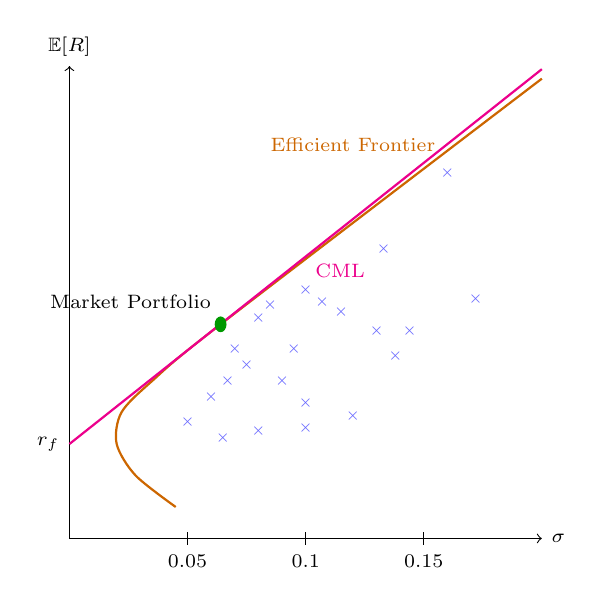
\begin{tikzpicture}[xscale=30, yscale=40]
        \draw[->] (0,0) -- (0.2,0) node[right] {\scriptsize $\sigma$};
        \draw[->] (0,0) -- (0,0.15) node[above] {\scriptsize $\E[R]$};
        \foreach \x in {0.05,0.1,0.15}{\draw (\x,0.002) -- (\x,-0.002) node[below] {\scriptsize \x};}
        \foreach \p in {(0.05,0.037),(0.06,0.045),(0.067,0.05),(0.07,0.06),(0.075,0.055),(0.08,0.07),(0.085,0.074),(0.09,0.05),(0.095,0.06),(0.1,0.079),(0.1,0.043),(0.107,0.075),(0.115,0.072),(0.12,0.039),(0.13,0.066),(0.133,0.092),(0.138,0.058),(0.144,0.066),(0.16,0.116),(0.172,0.076),(0.1,0.035),(0.08,0.034),(0.065,0.032)}
            {\node[blue!60,font=\tiny] at \p {$\times$};}
        \draw[thick,orange!80!black] plot[smooth] coordinates {(0.045,0.01) (0.028,0.02) (0.02,0.03) (0.022,0.04) (0.035,0.05) (0.064,0.068) (0.2,0.146)};
        \draw[thick,magenta] (0,0.03) -- (0.2,0.149);
        \fill[green!60!black] (0.064,0.068) circle (0.0025);
        \node[left,font=\scriptsize] at (0,0.03) {$r_f$};
        \node[above left,font=\scriptsize] at (0.064,0.07) {Market Portfolio};
        \node[font=\scriptsize,orange!80!black] at (0.12,0.125) {Efficient Frontier};
        \node[font=\scriptsize,magenta,right] at (0.1,0.085) {CML};
    \end{tikzpicture}
\end{center}
\begin{itemize}
    \item \rb{Efficient frontier}: the best expected return achievable for each volatility using portfolios of risky assets
    \item \rb{Capital market line (CML)}: the line from $r_f$ tangent to the frontier. The tangent point is the \rb{market portfolio (MP)}
    \item Mixing the MP with lending/borrowing at $r_f$ reaches any point on the CML, which beats the frontier everywhere else
\end{itemize}

\begin{example}[Leveraging Up the CML]
    $r_f = 3\%$, $\E[R_{MP}] = 7\%$, $\sigma_{MP} = 0.06$. Invest \$100 in the
    MP, then borrow another \$50 at $r_f$ and invest it in the MP too.
    \\\db{You hold 1.5$\times$ your wealth in the MP:}
    \[\sigma_p = 1.5\,\sigma_{MP} = 0.09, \qquad \E[R_p] = 1.5(7\% - 3\%) + 3\% = \db{9\%}\]
\end{example}

\heading{Systematic vs.\ Idiosyncratic Risk}
Regress a company's return on the market's:
\[R_{C,t} = \alpha_C + \beta_C' R_{MP,t} + \varepsilon_{C,t}\]
\begin{itemize}
    \item Volatility in $R_{MP,t}$ is \rb{systematic} (``market'') risk
    \item Volatility in $\varepsilon_{C,t}$ is \rb{idiosyncratic} (``firm-specific'') risk
    \item Investors can ``diversify away'' idiosyncratic risk with portfolios, so there is \b{no reward} for bearing it. Investors are only rewarded for market risk, measured by $\beta$
\end{itemize}

\begin{definition}[CAPM]
    The expected return of the $i$-th asset is
    \[\boxed{\E[R_i] = r_f + \beta_i\big(\E[R_{MP}] - r_f\big)}, \qquad
    \beta_i = \frac{\sigma_{i,MP}}{\sigma_{MP}^2} = \frac{\rho_{i,MP}\,\sigma_i}{\sigma_{MP}}\]
    $\E[R_{MP}] - r_f$ is the \rb{market risk premium}. The MP is often
    estimated with a stock index.
\end{definition}

\begin{center}
    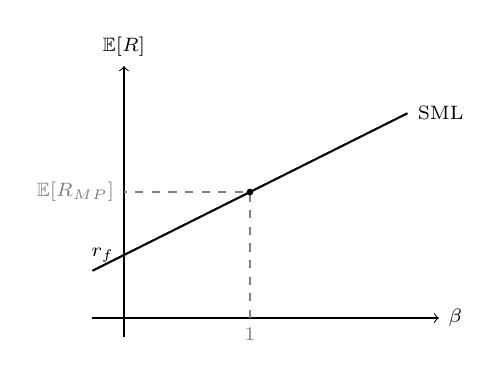
\begin{tikzpicture}[scale=0.8]
        \draw[->] (-0.5,0) -- (5,0) node[right] {\scriptsize $\beta$};
        \draw[->] (0,-0.3) -- (0,4) node[above] {\scriptsize $\E[R]$};
        \draw[thick] (-0.5,0.75) -- (4.5,3.25) node[right] {\scriptsize SML};
        \node[left] at (0,1) {\scriptsize $r_f$};
        \draw[dashed,gray] (2,0) node[below] {\scriptsize 1} -- (2,2) -- (0,2) node[left] {\scriptsize $\E[R_{MP}]$};
        \fill (2,2) circle (1.5pt);
    \end{tikzpicture}
    \\[2pt] \textit{\small Security market line: intercept $r_f$, slope $\E[R_{MP}] - r_f$}
\end{center}

\begin{example}[Estimating Stock Return]
    Market: $r_f = 2\%$, $\E[R_{MP}] = 8\%$, $\sigma_{MP} = 10\%$. Company X:
    correlation to the market $0.6$, volatility $0.15$. Estimate X's
    expected return.
    \[\beta_X = \frac{0.6 \times 0.15}{0.10} = 0.9\]
    \[\E[R_X] = 2\% + 0.9(8\% - 2\%) = \db{7.4\%}\]
    \db{(The handwritten slide used 10\% for the market return, giving 9.2\%. With the stated 8\% it is 7.4\%.)}
\end{example}

\begin{example}[Estimating Future Stock Price]
    A company with $\beta = 0.9$ trades at \$170/share. $r_f = 2\%$, market
    rate $= 7\%$. What is the expected share price in 5 years if it pays no
    dividends?
    \[\E[R_C] = 2\% + 0.9(7\% - 2\%) = 6.5\%\]
    \[P_5 = P_0 e^{\E[R_C]\,t} = 170e^{0.065 \times 5} = \db{\$235}\]
\end{example}

\begin{example}[Reflection: Stock with Dividends]
    A stock trades at \$10 and pays quarterly dividends of \$0.10/share.
    $\E[R_{MP}] = 10\%$, $r_f = 3\%$, $\beta = 1.2$. What is the expected
    price 3 years from now?
    \[\E[R_C] = 3\% + 1.2(10\% - 3\%) = 11.4\%/\text{yr}\]
    \db{Dividends are quarterly, so convert: $(1 + i_q)^4 = 1.114 \Rightarrow i_q = 2.736\%$. Today's price is the PV of 12 dividends plus the price at year 3:}
    \[10 = 0.10(P/A,2.736\%,12) + P_3(P/F,11.4\%,3) \;\Rightarrow\; P_3 = \db{\$12.43}\]
\end{example}

\topic{Arbitrage}

\begin{definition}[Arbitrage]
    \begin{itemize}
        \item \b{In financial markets}: taking advantage of a price difference between two or more markets
        \item \b{Academic use}: an opportunity to achieve a \b{risk-free} gain at a rate \b{greater than the risk-free rate}
        \item \rb{Statistical arbitrage}: a gain at a higher rate than one should get for a given level of risk
    \end{itemize}
    Fundamental to finance theory (and to valuation) is the
    \rb{no-arbitrage assumption}: ``no free lunch''.
\end{definition}

\begin{example}[Corn Arbitrage]
    You can buy a bushel of corn for \$10 today and enter a forward contract
    to deliver it for \$12 one year from now (storage is free). You can also
    borrow at 10\%. What would you do?
    \\\db{Borrow $\$10x$ and buy $x$ bushels today: net cash-flow \$0. In one year, sell the $x$ bushels for $\$12x$ and repay the $\$11x$ loan: a risk-free profit of $\$1x$.}
    \\\db{As $x \to \infty$ the profit is infinite. In reality, demand for corn today pushes the price up until the arbitrage disappears. The no-arbitrage price is}
    \[\frac{\$12}{1.10} = \db{\$10.91}\]
\end{example}

\heading{Futures and Forwards}
\begin{itemize}
    \item Contracts used to \b{hedge} against risks or to \b{speculate}
    \item Examples of \rb{derivative} assets: their value derives from an underlying asset
    \item Both lock in a specific price for a certain asset
\end{itemize}

\begin{definition}[Forward Contract]
    An obligation to buy or sell a certain asset at a specified price (the
    \rb{forward price}) at a specified time (the \rb{maturity} or expiration
    date). Typically not traded on exchanges; both buyer and seller are
    obligated to fulfill their end at maturity.
\end{definition}

\begin{definition}[Futures Contract]
    The same as a forward, except futures are \b{settled daily} (so they can
    be bought or sold at any time) and are traded on a \b{standardized
    exchange}.
\end{definition}

\begin{center}
    \begin{tabular}{ll}
        \toprule
        Futures & Forwards \\
        \midrule
        Settled daily & Settled at maturity \\
        Standardized & Not standardized \\
        Low risk of non-fulfilment (regulated) & Low regulation/oversight on settlement \\
        Traded on public exchanges & Private contract between two parties \\
        \bottomrule
    \end{tabular}
\end{center}
\db{E.g.\ the WTI oil futures curve: the price today for oil delivered in month 1, 2, \dots\ (in March 2020 the curve rose steeply from \$25 to \$45).}

\begin{example}[Interest Rate Forward]
    Given a yield curve $r(t)$, find the forward rate $r_{1,2}$ that one
    could lock in today for borrowing/lending from $t_1$ to $t_2$.
    \\\db{Invest $P_0$ today. Directly to $t_2$: $F_2 = P_0e^{r_{0,2}t_2}$. Or to $t_1$ then roll at the forward rate: $F_2' = P_0e^{r_{0,1}t_1}e^{r_{1,2}(t_2 - t_1)}$. No arbitrage requires $F_2' = F_2$:}
    \[\boxed{r_{1,2} = \frac{r_{0,2}t_2 - r_{0,1}t_1}{t_2 - t_1}}\]
\end{example}

\begin{example}[Foreign Exchange Forward]
    Canadian risk-free rate 3\%, US risk-free rate 2.5\%, current
    FX $= 0.9$ US\$/C\$. What is the fair one-year forward FX rate?
    \\\db{Two risk-free ways to turn C\$1 today into money in one year must agree:}
    \begin{itemize}
        \item \db{Keep it in C\$: $1 \times 1.03 = \text{C}\$1.03$}
        \item \db{Convert to US\$0.90, invest: $0.90 \times 1.025 = \text{US}\$0.9225$}
    \end{itemize}
    \[FX_1 = \frac{\text{US}\$0.9225}{\text{C}\$1.03} = \db{0.896 \text{ US\$/C\$}}\]
\end{example}

\heading{Using Replication to Price an Asset}
Build a portfolio of assets we can already price that has the \b{same
payoff in every state}. By no-arbitrage, the asset's price equals the
portfolio's price.

\begin{example}[Pricing a Project by Replication]
    A project pays \$140 if the market goes up and \$30 if it goes down.
    The risk-free rate is 5\% for the period; the MP is \$100 today and will be
    worth \$120 (up) or \$95 (down). What is a fair price for the project?
    \begin{center}
        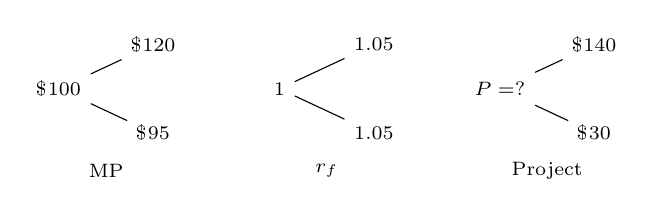
\begin{tikzpicture}[scale=0.8, every node/.style={font=\scriptsize}]
            \node (m) at (0,0) {\$100}; \node (mu) at (1.5,0.7) {\$120}; \node (md) at (1.5,-0.7) {\$95};
            \draw (m) -- (mu); \draw (m) -- (md); \node at (0.75,-1.3) {MP};
            \node (r) at (3.5,0) {1}; \node (ru) at (5,0.7) {1.05}; \node (rd) at (5,-0.7) {1.05};
            \draw (r) -- (ru); \draw (r) -- (rd); \node at (4.25,-1.3) {$r_f$};
            \node (p) at (7,0) {$P = ?$}; \node (pu) at (8.5,0.7) {\$140}; \node (pd) at (8.5,-0.7) {\$30};
            \draw (p) -- (pu); \draw (p) -- (pd); \node at (7.75,-1.3) {Project};
        \end{tikzpicture}
    \end{center}
    \db{Hold $a$ units of the MP and $b$ units of the risk-free asset:}
    \begin{align*}
        \text{Up: } & 120a + 1.05b = 140\\
        \text{Down: } & 95a + 1.05b = 30
    \end{align*}
    \db{$\Rightarrow a = 4.4$, $b = -369.52$ (borrow).}
    \[P = 100(4.4) - 1(369.52) = \db{\$70.48}\]
    \db{Note that we did \dbb{not} use the probabilities!}
\end{example}

\begin{example}[Expected Returns and the Project's Beta]
    Same setup; the probability the market goes up is 60\%.
    \[\E[R_{MP}] = \frac{120(0.6) + 95(0.4)}{100} - 1 = 10\%\]
    \[\E[R_{proj}] = \frac{140(0.6) + 30(0.4)}{70.48} - 1 = 36.2\%\]
    \db{Back out the project's beta from CAPM:}
    \[36.2\% = 5\% + \beta_{proj}(10\% - 5\%) \;\Rightarrow\; \beta_{proj} = \db{6.24}\]
    \db{The project swings far more than the market, so it is heavily ``leveraged'' market risk.}
\end{example}

\begin{example}[Payoffs Independent of the Market]
    \begin{enumerate}[label = \alph*)]
        \item What if the project paid \$140 regardless of what the market did?
        \\\db{It is risk-free: $P = 140/1.05 = \$133$.}
        \item What if the payoff had a 50\% chance of being \$150 and 50\% of being \$130 (independent of the market)?
        \\\db{$\E[\text{payoff}] = 0.5(150) + 0.5(130) = \$140$. The risk is purely idiosyncratic (diversifiable), so it carries no premium: $P = 140/1.05 = \$133$.}
    \end{enumerate}
\end{example}

\begin{example}[Systematic and Idiosyncratic Risk]
    A wealthy (risk-neutral) investor can invest in a product development
    project. There is a 60\% chance the technology works very well
    (independent of the market). Payoffs:
    \begin{center}
    \begin{tabular}{lcc}
        \toprule
        & Tech works (60\%) & Doesn't (40\%) \\
        \midrule
        Market up & \$80k & \$50k \\
        Market down & \$55k & \$20k \\
        \bottomrule
    \end{tabular}
    \end{center}
    The MP is \$45 today, worth \$60 (up) or \$40 (down); $r_f = 5\%$. An
    initial R\&D investment of \$20k is required. What is the maximum price
    for the project?
    \\\db{The technology risk is idiosyncratic, so replace it by its expectation in each market state:}
    \[\E[P_u] = 0.6(80k) + 0.4(50k) = 68k, \qquad \E[P_d] = 0.6(55k) + 0.4(20k) = 41k\]
    \db{Replicate the market risk:}
    \begin{align*}
        60a + 1.05b &= 68k\\
        40a + 1.05b &= 41k
    \end{align*}
    \db{$\Rightarrow a = 1.35k$, $b = -12.38k$.}
    \[P_0 = 1.35k(45) - 12.38k = \$48.37k\]
    \db{Since \$20k of R\&D is also needed, buy the project for \dbb{\$28.37k or less}.}
\end{example}

\begin{example}[Bond: Accounting for Default]
    A company issues a 5-year bond (face \$100) with a 5\% annual coupon.
    The \b{risk-neutral probability} of default in any given year is 5\%,
    and on default only half of the principal (\$50) is paid out. The
    risk-free rate is 3\%.
    \begin{enumerate}[label = \alph*)]
        \item What is the probability of default over the 5 years?
        \\\db{$1 - 0.95^5 = 22.6\%$}
        \item What should the price of the bond be?
        \\\db{Work backwards through the tree. Each year the bond either survives (95\%, pays the coupon plus the value going forward) or defaults (5\%, pays \$50). Discount each step at $r_f$ since these are risk-neutral probabilities:}
        \begin{align*}
            P_{up}^{(4)} &= 5 + \frac{0.95(105) + 0.05(50)}{1.03} = 104.27\\
            P_{up}^{(3)} &= 5 + \frac{0.95(104.27) + 0.05(50)}{1.03} = 103.60\\
            P_{up}^{(2)} &= 5 + \frac{0.95(103.60) + 0.05(50)}{1.03} = 102.98\\
            P_{up}^{(1)} &= 5 + \frac{0.95(102.98) + 0.05(50)}{1.03} = 102.41\\
            P_0 &= \frac{0.95(102.41) + 0.05(50)}{1.03} = \db{\$96.88}
        \end{align*}
        \item What is the yield?
        \[96.88 = 5(P/A,y,5) + 100(P/F,y,5) \;\Rightarrow\; y = \db{5.735\%}\]
        \db{The yield is above the 3\% risk-free rate (and the 5\% coupon) to compensate for default risk.}
    \end{enumerate}
\end{example}

\heading{Summary}
\begin{enumerate}
    \item Risk is the uncertainty in a future payoff; investors demand a higher expected return for bearing it
    \item Only \b{systematic} (market) risk is rewarded. CAPM: $\E[R_i] = r_f + \beta_i(\E[R_{MP}] - r_f)$
    \item \b{No arbitrage}: two ways to get the same payoff must cost the same. This prices forwards (corn, interest rates, FX)
    \item \b{Replication}: match an asset's payoffs with the MP and the risk-free asset; the price does not need the real-world probabilities
\end{enumerate}


\end{document}
